\documentclass[12pt]{article}

\usepackage{hcmus-report-template}
\usepackage{longtable}
\usepackage{booktabs}
\usepackage{enumitem}

% Disable indentation on new paragraphs
\setlength{\parindent}{0pt}

% Line spacing 1.5
\renewcommand{\baselinestretch}{1.5}

% Graphic path
\graphicspath{{img/}}

% Define course name, report name and report title.
\newcommand{\coursename}{DevOps}
\newcommand{\reportname}{Triển khai hệ thống CI cho dự án YAS}
\newcommand{\reporttitle}{Đồ án 1: Triển khai hệ thống CI}

\newcommand{\studentname}{%
Nguyễn Lê Thế Vinh (MSSV1)\\
Phạm Quang Vinh (MSSV2)\\
Lê Xuân Trí (MSSV3)%
}
\newcommand{\teachername}{[Tên giảng viên]}

% Header
\lhead{\reporttitle}
\rhead{
Trường Đại học Khoa học Tự nhiên - ĐHQG HCM\\
\coursename
}

% Footer
\newcommand{\leftfooter}{YAS CI/CD Pipeline Report}
\lfoot{\leftfooter}

% ============ DOCUMENT ============
\begin{document}

\pagenumbering{roman}
\input{content/title.tex}

\tableofcontents
\pagebreak

\pagenumbering{arabic}
\setcounter{page}{1}

% Nội dung báo cáo
\section{Tổng quan dự án}

\subsection{Giới thiệu YAS}
YAS (\textit{Yet Another Shop}) là một dự án mã nguồn mở được phát triển bởi NashTech Garage, nhằm mục đích xây dựng một ứng dụng thương mại điện tử microservice điển hình bằng Java/Spring Boot.

Dự án sử dụng kiến trúc \textbf{monorepo} --- tất cả các service được quản lý trong một repository duy nhất, bao gồm hơn 19 module:
\begin{itemize}[noitemsep]
    \item \textbf{Business Services}: media, product, cart, order, rating, customer, location, inventory, tax, search, payment, promotion, recommendation, delivery, webhook, sampledata
    \item \textbf{BFF (Backend-for-Frontend)}: storefront-bff, backoffice-bff
    \item \textbf{Shared Library}: common-library
\end{itemize}

\subsection{Mục tiêu đồ án}
Xây dựng hệ thống \textbf{Continuous Integration (CI)} cho dự án YAS bằng Jenkins, đáp ứng các yêu cầu:
\begin{enumerate}[noitemsep]
    \item Sử dụng Jenkins làm CI server
    \item Fork repo và cấu hình branch protection
    \item Pipeline có ít nhất 2 phase: test và build
    \item Monorepo path filter --- chỉ build/test service thay đổi
    \item Coverage gate $\geq$ 70\%
    \item Security scanning: Gitleaks, SonarQube, Snyk
\end{enumerate}

\subsection{Công nghệ sử dụng}
\begin{table}[H]
\centering
\caption{Công nghệ và công cụ sử dụng}
\begin{tabular}{|l|l|l|}
\hline
\textbf{Thành phần} & \textbf{Công nghệ} & \textbf{Phiên bản} \\
\hline
Ngôn ngữ & Java & 21 \\
\hline
Framework & Spring Boot & 3.2 \\
\hline
Build tool & Maven & Latest LTS \\
\hline
CI Server & Jenkins & 2.555.1 \\
\hline
Code hosting & GitHub & --- \\
\hline
JDK (Jenkins) & OpenJDK & 25 \\
\hline
Secret scanning & Gitleaks & 8.18.4 \\
\hline
Code quality & SonarQube & Self-hosted \\
\hline
Dependency scan & Snyk & CLI \\
\hline
Coverage tool & JaCoCo & 0.8.14 \\
\hline
Infrastructure & AWS EC2 & --- \\
\hline
\end{tabular}
\end{table}

\subsection{Thông tin repository}
\begin{itemize}[noitemsep]
    \item \textbf{Repository gốc}: \url{https://github.com/nashtech-garage/yas}
    \item \textbf{Repository nhóm (fork)}: \url{https://github.com/tzin1401/yas}
    \item \textbf{Jenkins}: \url{http://3.27.92.213:8080}
    \item \textbf{SonarQube}: \url{http://3.27.92.213:9000}
\end{itemize}

\section{Kiến trúc hệ thống CI}

\subsection{Tổng quan kiến trúc}
Hệ thống CI được thiết kế với luồng hoạt động như sau:

\begin{enumerate}[noitemsep]
    \item Developer tạo branch mới, viết code và push lên GitHub
    \item Developer tạo Pull Request (PR) vào branch \texttt{main}
    \item GitHub Webhook tự động thông báo Jenkins
    \item Jenkins Multibranch Pipeline tự động phát hiện và chạy pipeline
    \item Pipeline thực thi 8 stages tuần tự
    \item Kết quả CI được báo về GitHub qua commit status
    \item PR chỉ được merge khi CI pass và có đủ 2 reviewer approve
\end{enumerate}

\subsection{Sơ đồ luồng CI}
Luồng CI pipeline bao gồm 8 stages chính:

\begin{table}[H]
\centering
\caption{8 Stages của CI Pipeline}
\begin{tabular}{|c|l|l|}
\hline
\textbf{Stage} & \textbf{Tên} & \textbf{Mô tả} \\
\hline
1 & Checkout & Clone code, fetch origin/main \\
\hline
2 & Detect Changed Modules & Xác định modules thay đổi (monorepo filter) \\
\hline
3 & Gitleaks -- Secret Scan & Quét secrets/API keys rò rỉ \\
\hline
4 & Test & Chạy unit tests + JaCoCo coverage report \\
\hline
5 & Coverage Gate & Kiểm tra coverage $\geq$ 70\% \\
\hline
6 & Build & Build các modules thay đổi \\
\hline
7 & SonarQube -- Analysis & Phân tích chất lượng code \\
\hline
8 & Snyk -- Dependency Scan & Quét lỗ hổng dependencies \\
\hline
\end{tabular}
\end{table}

\subsection{Hạ tầng và Kiến trúc Build phân tán (Master-Agent)}
\begin{itemize}[noitemsep]
    \item \textbf{Jenkins Server (Master node)}: Đóng vai trò làm máy chủ trung tâm (Orchestrator). Nhiệm vụ duy nhất là tiếp nhận tín hiệu từ GitHub Webhook, lập lịch, quản lý cấu hình Pipeline, lưu trữ lịch sử build và phân phối tác vụ xuống các Agent.
    \item \textbf{SonarQube Server}: Triển khai độc lập để phân tích chất lượng code của toàn bộ dự án.
    \item \textbf{Distributed Agents (Cộng tác viên build)}: Toàn bộ quá trình checkout code, build, unit test và phân tích bảo mật được giao hoàn toàn cho 3 Agent thực thi song song:
    \begin{itemize}[noitemsep]
        \item \textbf{Agent-Tri}: Phụ trách xử lý và thực thi các build job.
        \item \textbf{Agent-QVinh}: Phụ trách xử lý và thực thi các build job.
        \item \textbf{Agent-TVinh}: Phụ trách xử lý và thực thi các build job.
    \end{itemize}
    \item \textbf{Lợi ích}: Phân tán tải công việc giúp ngăn chặn tình trạng thắt nút cổ chai (bottleneck) tại Master node, đồng thời giúp tăng tốc thời gian hoàn thành pipeline lên gấp nhiều lần.
\end{itemize}

\section{Cấu hình GitHub}

\subsection{Fork Repository}
Nhóm đã fork repository gốc \texttt{nashtech-garage/yas} về tài khoản \texttt{tzin1401/yas}. Tất cả thành viên được thêm làm collaborator với quyền write.

% [Ảnh: Screenshot GitHub repo tzin1401/yas]

\subsection{Branch Protection Rules (GitHub Rulesets)}
Để đảm bảo chất lượng code, nhóm đã cấu hình GitHub Rulesets cho branch \texttt{main} với các quy tắc:

\begin{enumerate}[noitemsep]
    \item \textbf{Không cho phép push trực tiếp}: Mọi thay đổi phải thông qua Pull Request
    \item \textbf{Yêu cầu tối thiểu 2 reviewer approve}: Đảm bảo code review đầy đủ
    \item \textbf{Required status check}: CI pipeline phải pass (\texttt{continuous-integration/jenkins/pr-head})
    \item \textbf{Không cho phép force push}: Bảo vệ lịch sử commit
\end{enumerate}

% [Ảnh: Screenshot GitHub Rulesets configuration]
% [Ảnh: Screenshot hiển thị "Review required" và "Checks" trên PR]

\subsection{Webhook GitHub → Jenkins}
Cấu hình webhook để GitHub tự động thông báo Jenkins khi có push hoặc PR:
\begin{itemize}[noitemsep]
    \item \textbf{Payload URL}: \texttt{http://3.27.92.213:8080/github-webhook/}
    \item \textbf{Content type}: \texttt{application/json}
    \item \textbf{Events}: Push events, Pull request events
\end{itemize}

% [Ảnh: Screenshot GitHub Webhook configuration]
% [Ảnh: Screenshot Webhook delivery history (Recent Deliveries)]

\subsection{Quy trình làm việc với Git}
Nhóm tuân theo quy trình Git Flow đơn giản:
\begin{enumerate}[noitemsep]
    \item Tạo branch mới từ \texttt{main} (ví dụ: \texttt{feature/media-tests}, \texttt{ci/setup-jenkins-pipeline})
    \item Phát triển và commit code trên branch
    \item Push branch lên GitHub
    \item Tạo Pull Request vào \texttt{main}
    \item Jenkins tự động chạy CI pipeline
    \item 2 thành viên khác review và approve
    \item Merge PR khi CI pass và đủ approvals
\end{enumerate}

\section{Cấu hình máy chủ và Môi trường hệ thống}
\label{sec:cau-hinh-server}

Để vận hành quy trình CI/CD hoàn chỉnh, nhóm đã triển khai một máy chủ riêng biệt trên nền tảng điện toán đám mây.

\subsection{Khởi tạo máy chủ trên AWS (EC2)}
Nhóm sử dụng dịch vụ Amazon EC2 để tạo máy chủ với các thông số sau:
\begin{itemize}[noitemsep]
    \item \textbf{Hệ điều hành}: Ubuntu Server 24.04 LTS (Hỗ trợ tốt nhất cho Docker)
    \item \textbf{Instance Type}: \texttt{t3.small} (2 vCPU, 2GB RAM).
    \item \textbf{Bộ nhớ mở rộng (Swap Memory)}: Cấu hình 4GB Swap để tránh tình trạng tràn bộ nhớ (Out-of-memory) khi SonarQube và Jenkins chạy đồng thời.
\end{itemize}

\begin{figure}[H]
    \centering
    % CHỈ DẪN ẢNH: Thả ảnh 01-aws-ec2-instances-list.png vào thư mục img/
    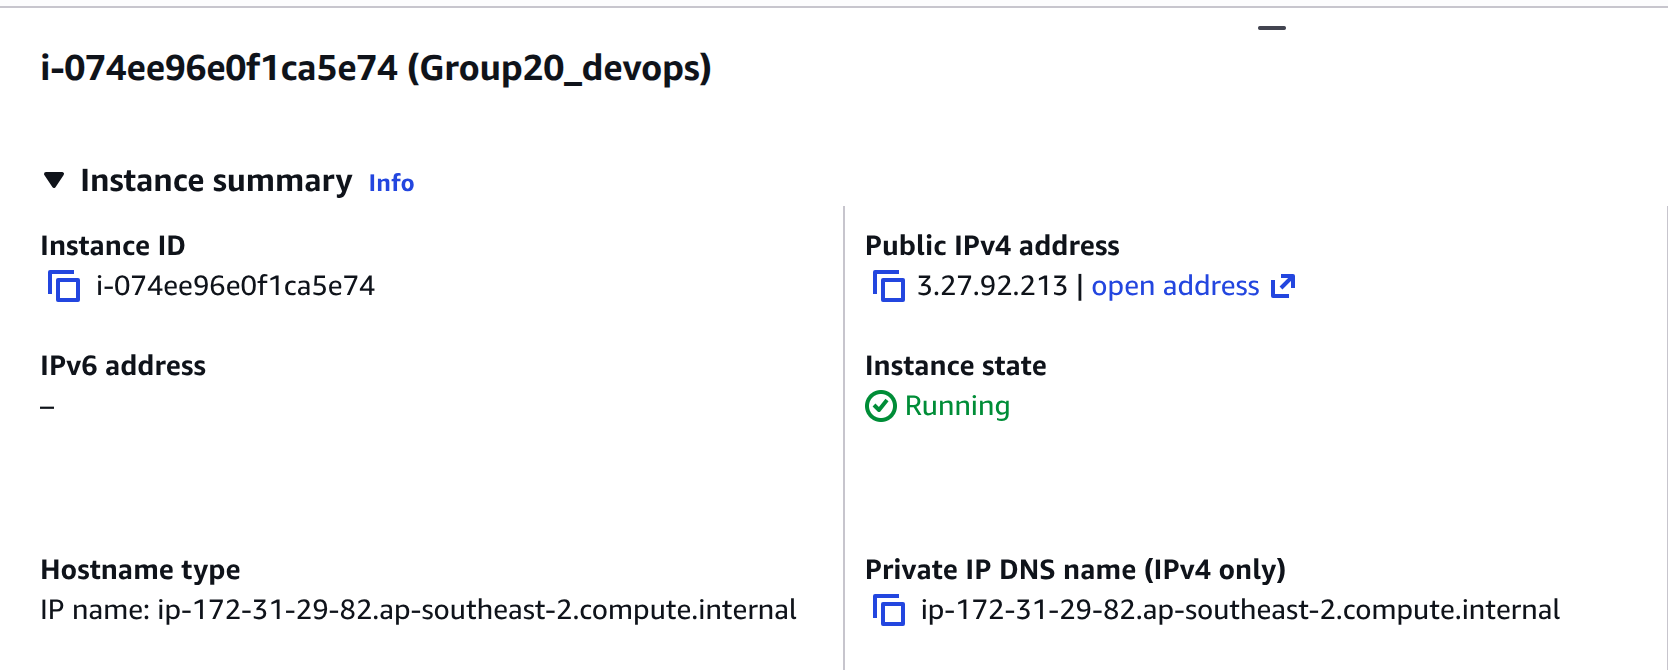
\includegraphics[width=0.9\textwidth]{img/01-aws-ec2-instances-list.png}
    \caption{Danh sách các máy chủ EC2 phục vụ hệ thống CI/CD}
\end{figure}

Trên AWS Console, nhóm tạo một Security Group và mở các cổng mạng thiết yếu (22, 8080, 9000, 50000).

\begin{figure}[H]
    \centering
    % CHỈ DẪN ẢNH: Thả ảnh 02-aws-security-group-rules.png vào thư mục img/
    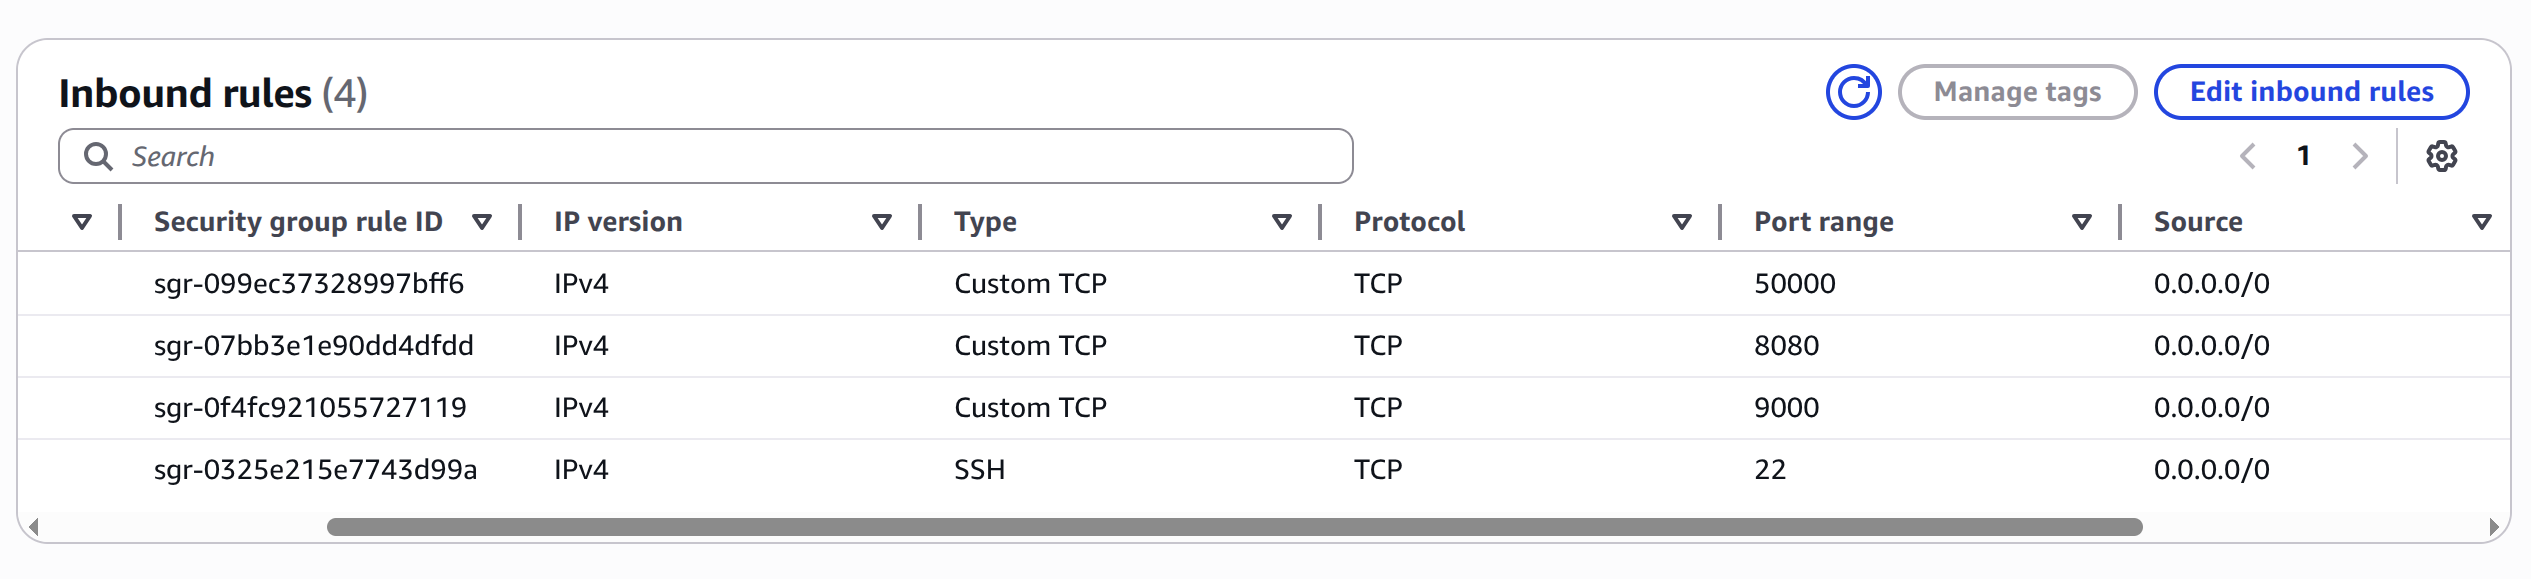
\includegraphics[width=0.9\textwidth]{img/02-aws-security-group-rules.png}
    \caption{Thiết lập quy tắc Inbound rules của Security Group}
\end{figure}

\subsection{Cài đặt và Quản trị môi trường Docker}
Dự án sử dụng công nghệ Container để cô lập môi trường và dễ dàng quản lý dịch vụ.

\textbf{Cài đặt Docker Engine}: Nhóm tiến hành cài đặt các gói \texttt{docker.io} và \texttt{docker-compose} trên nền tảng Ubuntu.

\begin{lstlisting}[language=bash, caption={Cài đặt Docker trên Ubuntu Server}]
# Cap nhat he thong
sudo apt update && sudo apt upgrade -y

# Cai dat Docker Engine
sudo apt install docker.io -y
sudo systemctl start docker
sudo systemctl enable docker

# Cap quyen chay Docker khong can sudo
sudo usermod -aG docker $USER

# Cai dat Docker Compose
sudo apt install docker-compose -y
\end{lstlisting}

\textbf{Thiết lập cấu hình triển khai (Docker Compose)}: Thay vì cài đặt rời rạc, dự án sử dụng Docker Compose để quản lý tập trung Jenkins và SonarQube.

\begin{lstlisting}[language=make, caption={Tệp cấu hình docker-compose.yml tiêu chuẩn}]
version: '3.8'
services:
  jenkins:
    image: jenkins/jenkins:lts
    container_name: jenkins
    ports:
      - "8080:8080"
      - "50000:50000"
    volumes:
      - jenkins_home:/var/jenkins_home
      - /var/run/docker.sock:/var/run/docker.sock
    restart: always

  sonarqube:
    image: sonarqube:lts-community
    container_name: sonarqube
    ports:
      - "9000:9000"
    environment:
      - SONAR_ES_BOOTSTRAP_CHECKS_DISABLE=true
    volumes:
      - sonarqube_data:/opt/sonarqube/data
    restart: always

volumes:
  jenkins_home:
  sonarqube_data:
\end{lstlisting}

\textbf{Quản trị bằng Docker CLI}: Thay vì cài đặt truyền thống, việc tương tác với dịch vụ được thực hiện qua các lệnh thực thi trực tiếp vào Container.

\textbf{Lấy mật khẩu Jenkins}: Sử dụng lệnh sau để lấy mã unlock hệ thống ban đầu:
\begin{lstlisting}[language=bash]
docker exec jenkins cat /var/jenkins_home/secrets/initialAdminPassword
\end{lstlisting}

\textbf{Kiểm tra trạng thái}: Sử dụng lệnh sau để xác nhận các container \texttt{jenkins} và \texttt{sonarqube} đang vận hành ổn định:
\begin{lstlisting}[language=bash]
docker ps
\end{lstlisting}

\begin{figure}[H]
    \centering
    % CHỈ DẪN ẢNH: Thả ảnh 03-docker-ps-status.png vào thư mục img/
    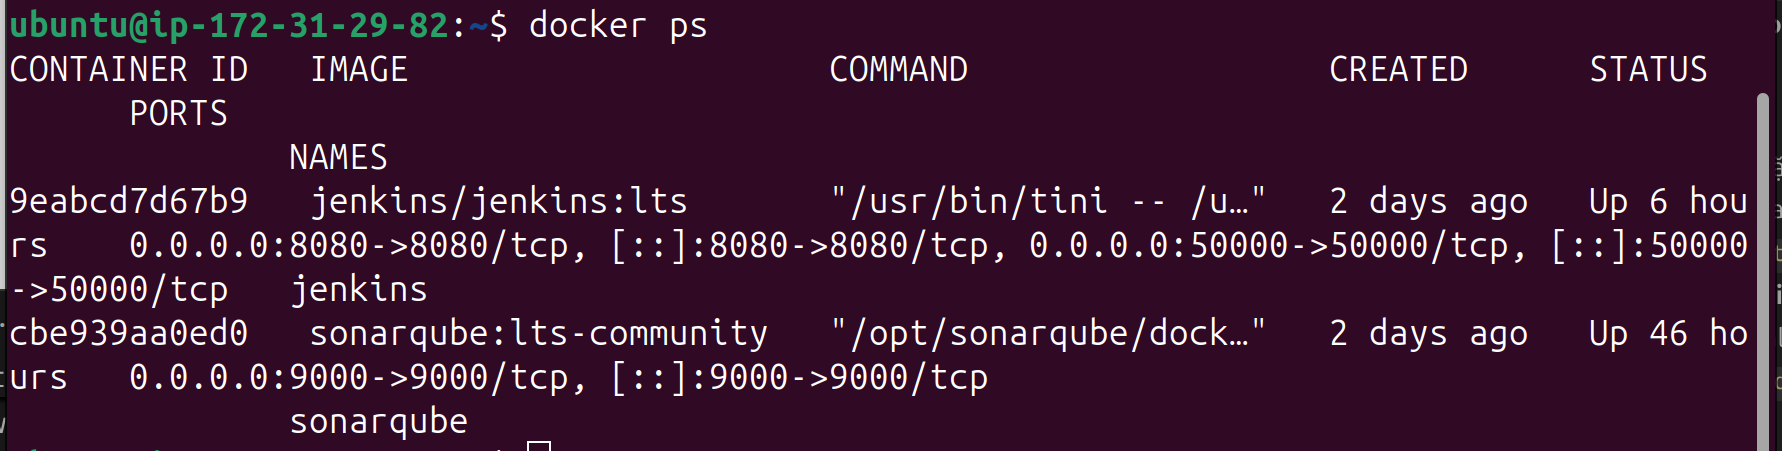
\includegraphics[width=0.9\textwidth]{img/03-docker-ps-status.png}
    \caption{Danh sách các container dịch vụ đang hoạt động ổn định}
\end{figure}

\subsection{Cấu hình tích hợp hệ thống (System Integration)}
Thiết lập luồng giao tiếp tự động giữa GitHub, Jenkins và SonarQube.

\textbf{GitHub Webhook}: Cấu hình Webhook trên Repository để gửi tín hiệu tới Jenkins mỗi khi có sự kiện Push hoặc Pull Request.

\begin{figure}[H]
    \centering
    % CHỈ DẪN ẢNH: Thả ảnh 05-github-webhook-config.png vào thư mục img/
    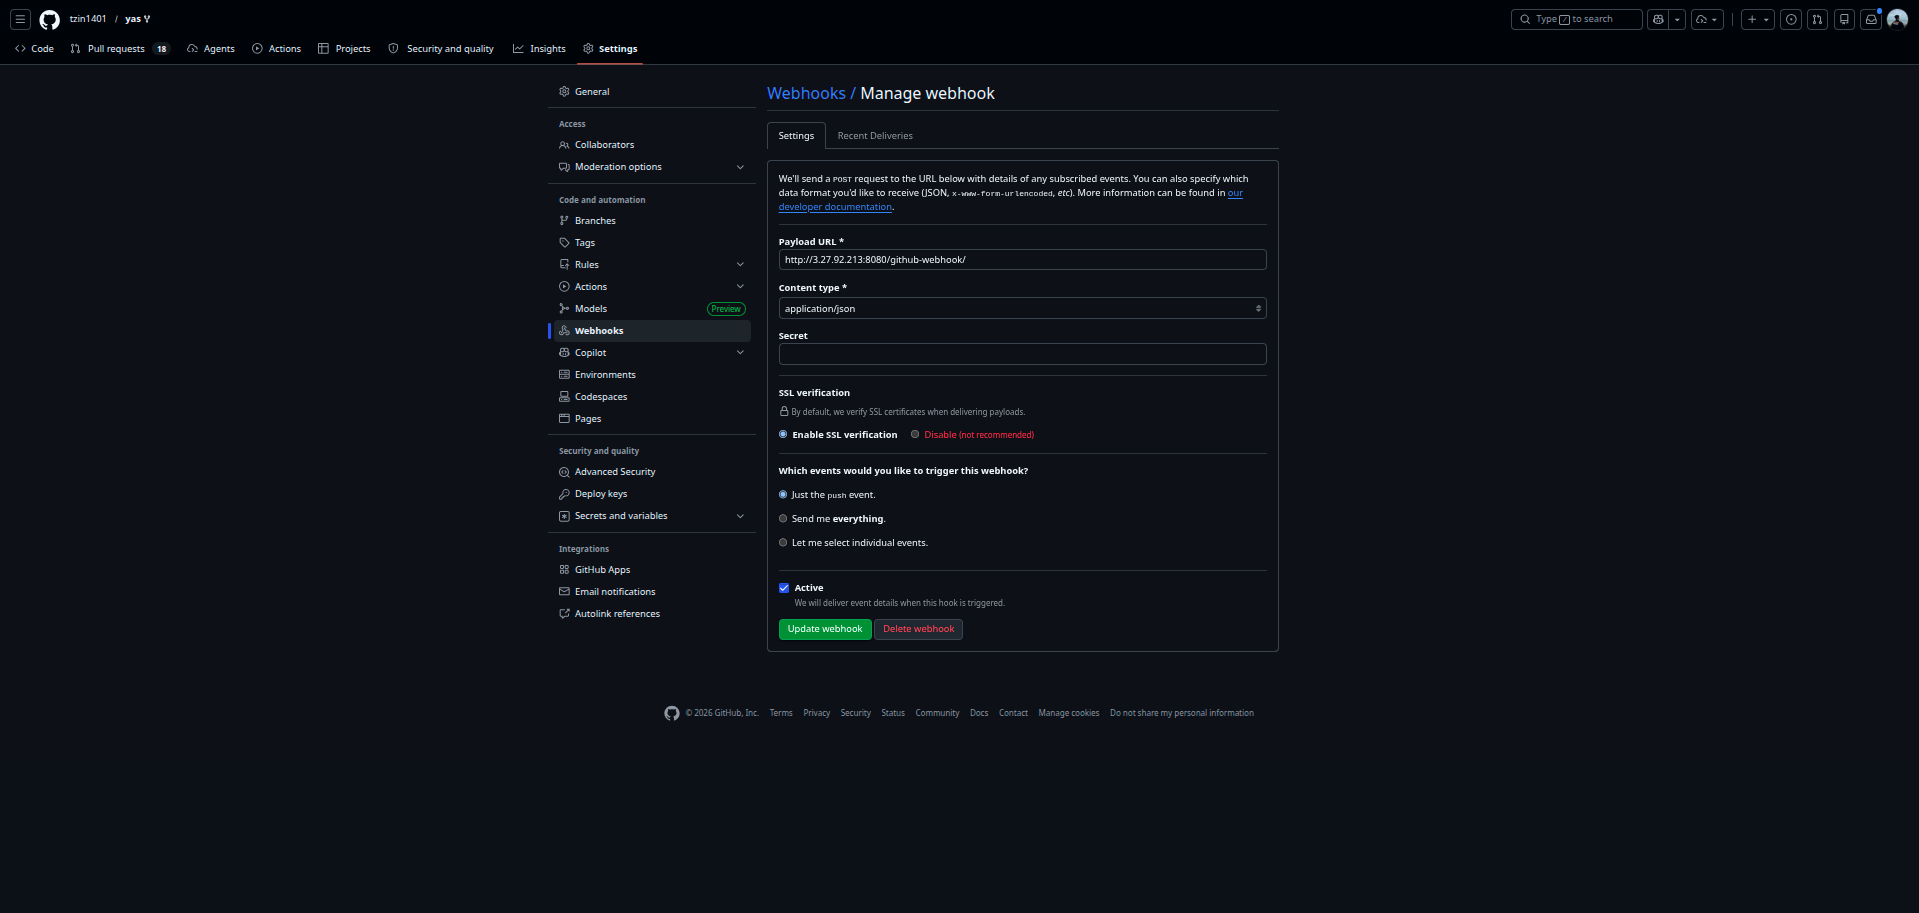
\includegraphics[width=0.9\textwidth]{img/03-github-webhook-list1.png}
    \caption{URL Webhook trên GitHub có dấu tích xanh (Active)}
\end{figure}

\textbf{SonarQube Webhook}: Cấu hình Webhook ngược từ SonarQube về Jenkins (\texttt{http://<IP-Jenkins>:8080/sonarqube-webhook/}) để trả kết quả Quality Gate.

\begin{figure}[H]
    \centering
    % CHỈ DẪN ẢNH: Thả ảnh 06-sonarqube-webhook-config.png vào thư mục img/
    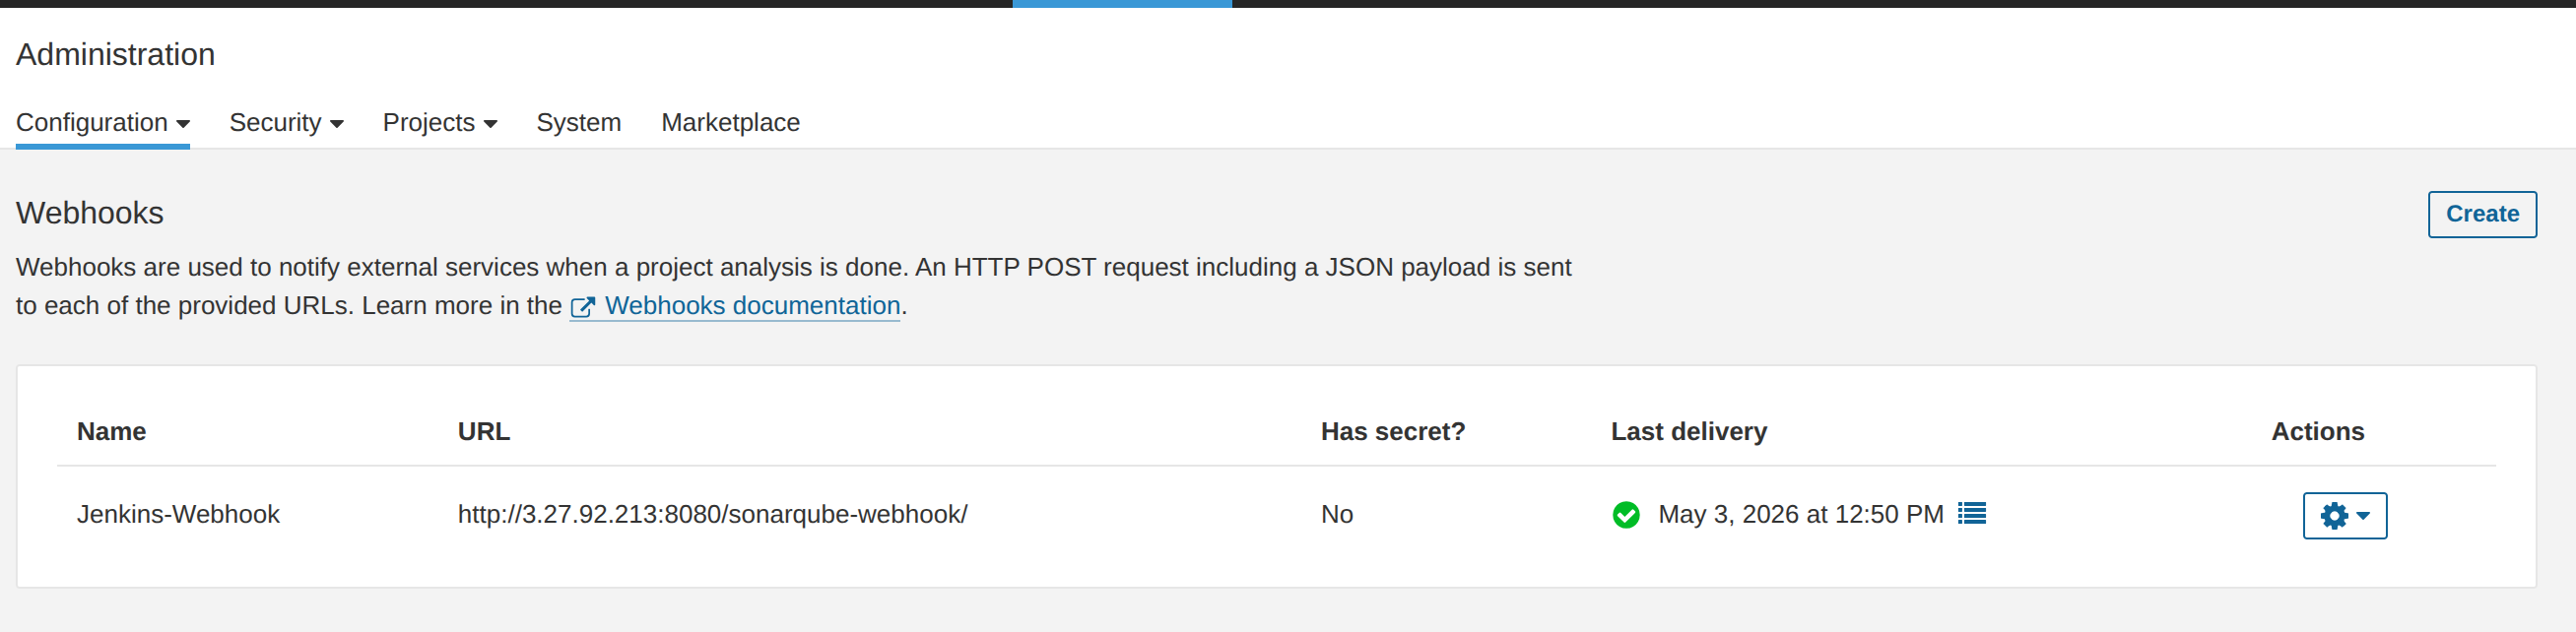
\includegraphics[width=0.9\textwidth]{img/06-sonarqube-webhook-config.png}
    \caption{Cấu hình Webhook gửi dữ liệu ngược từ SonarQube về lại Jenkins}
\end{figure}

\textbf{Quản lý thông tin bảo mật}: Thiết lập các ID Credentials trong Jenkins (\texttt{sonarqube-token}, \texttt{snyk-token}) để kết nối an toàn với các dịch vụ bên thứ ba.

\section{Cấu hình Jenkins}
\label{sec:cau-hinh-jenkins}

\subsection{Cài đặt Jenkins trên AWS EC2}
Jenkins được cài đặt trên AWS EC2 instance và truy cập qua \texttt{http://3.27.92.213:8080}.

Các plugin cần thiết đã cài đặt:
\begin{itemize}[noitemsep]
    \item \textbf{GitHub Branch Source Plugin}: Hỗ trợ Multibranch Pipeline với GitHub
    \item \textbf{Pipeline Plugin}: Hỗ trợ Jenkinsfile declarative pipeline
    \item \textbf{JUnit Plugin}: Hiển thị kết quả test
    \item \textbf{Credentials Binding Plugin}: Quản lý secrets (SonarQube token, Snyk token)
    \item \textbf{Timestamps Plugin}: Hiển thị thời gian trong console output
\end{itemize}

\begin{figure}[H]
    \centering
    % CHỈ DẪN ẢNH: Thả ảnh 01-jenkins-dashboard.png vào thư mục img/
    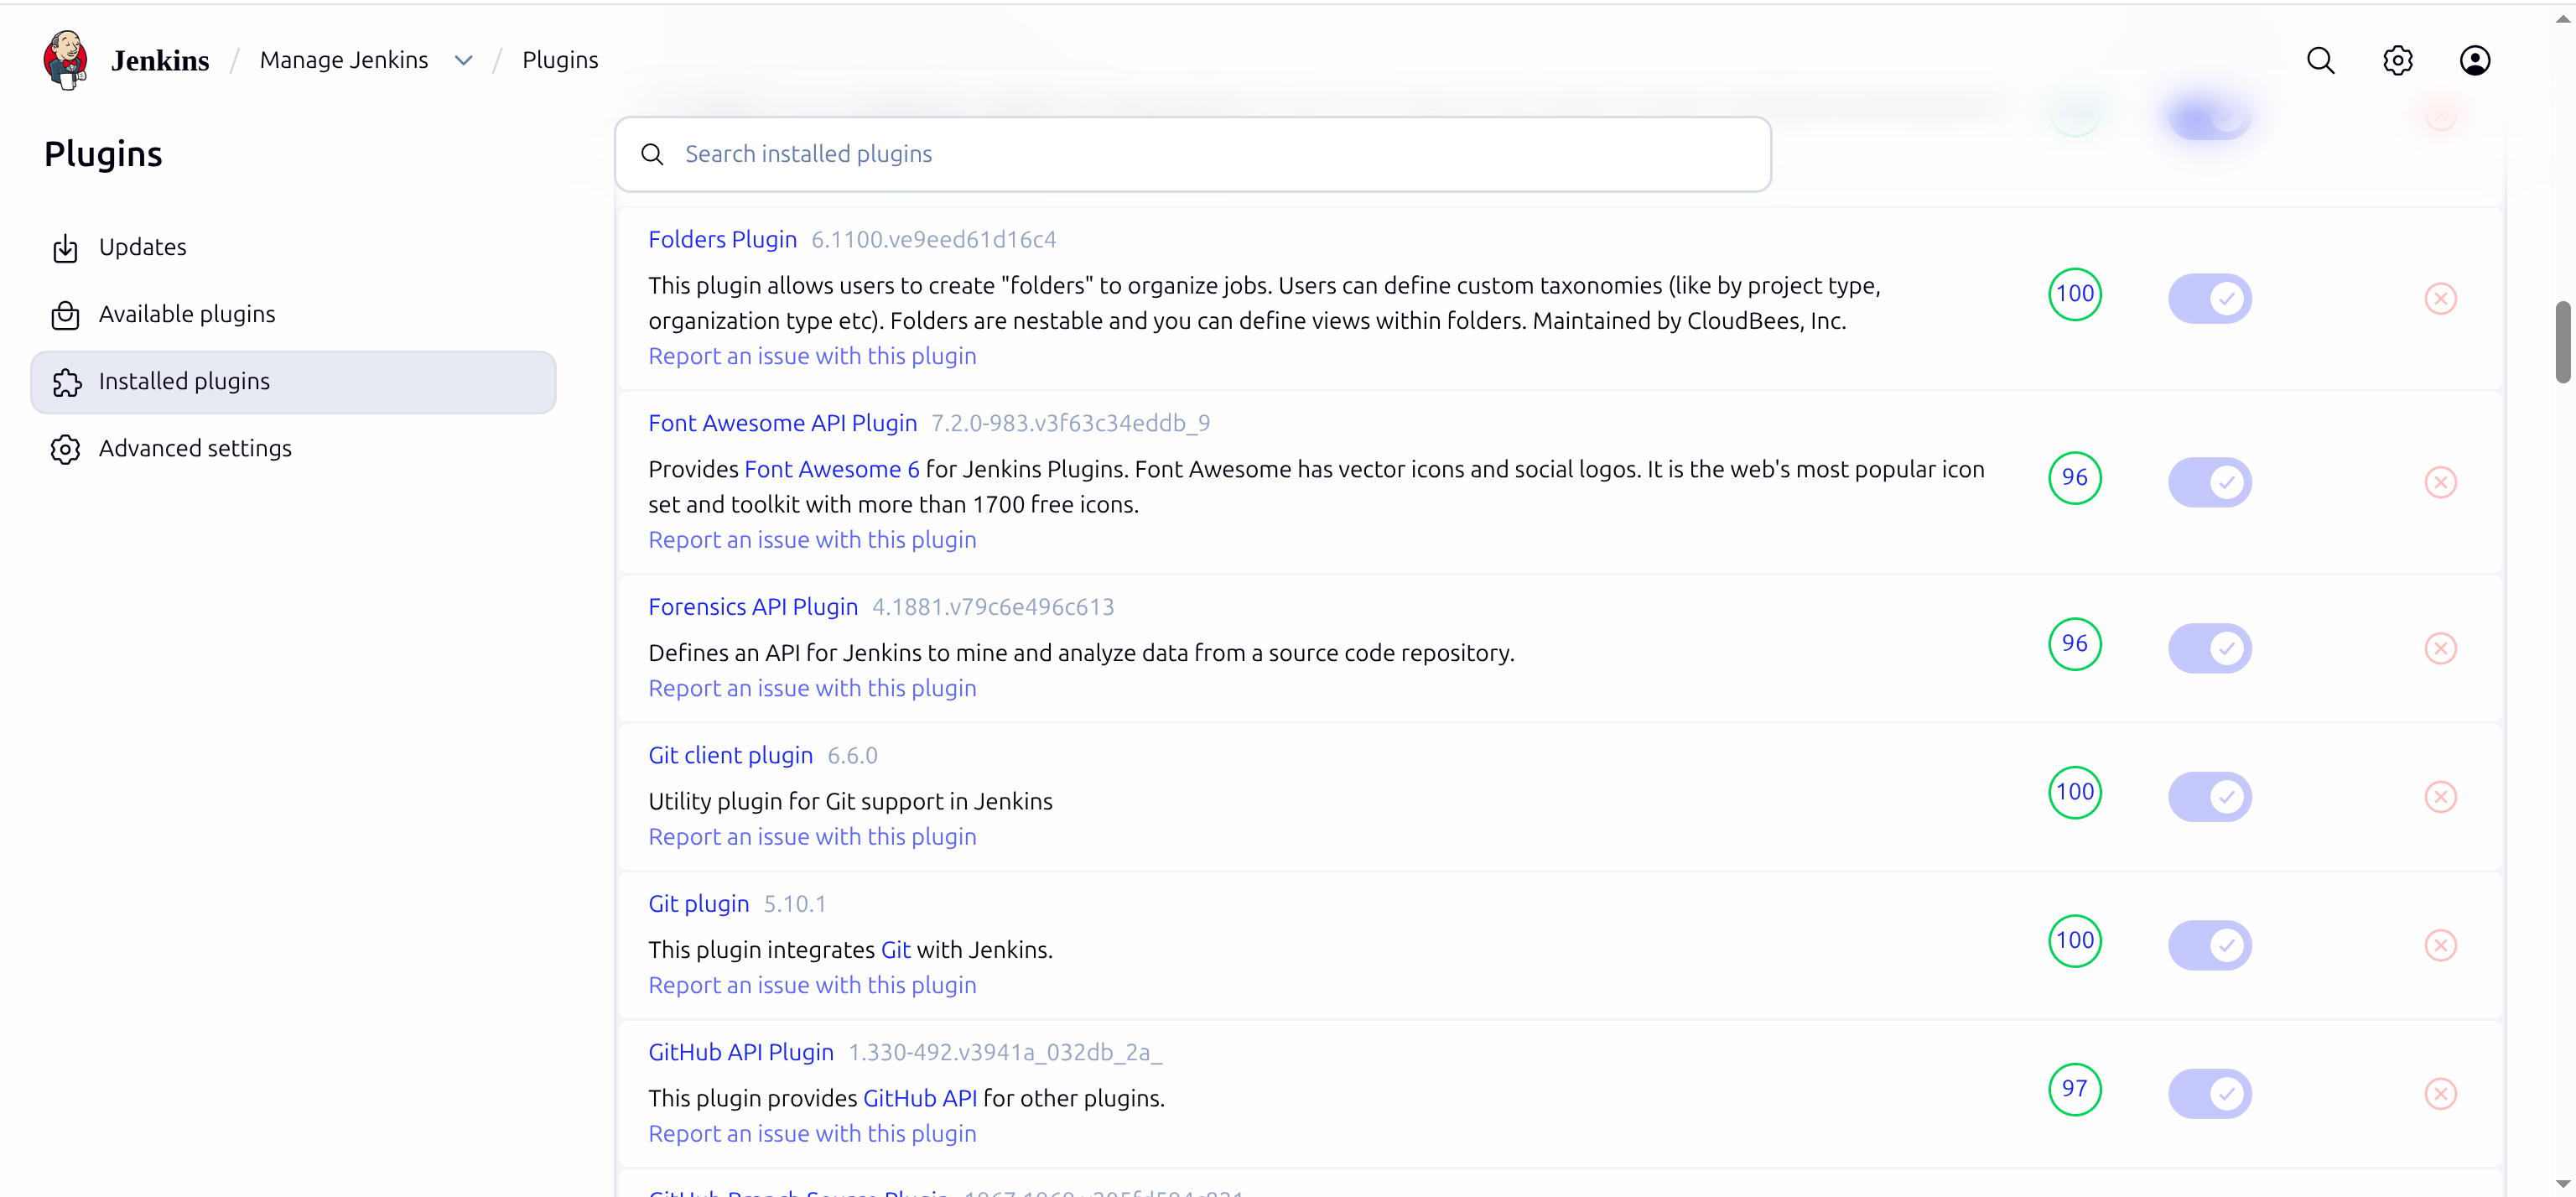
\includegraphics[width=0.9\textwidth]{img/01-jenkins-dashboard.png}
    \caption{Giao diện Dashboard quản lý Jenkins trên AWS EC2}
\end{figure}

\subsection{Cấu hình Tools}
Trong Jenkins Global Tool Configuration:
\begin{itemize}[noitemsep]
    \item \textbf{JDK}: Cấu hình JDK-25 (OpenJDK 25)
    \item \textbf{Maven}: Cấu hình Maven (Latest LTS)
\end{itemize}

\begin{figure}[H]
    \centering
    % CHỈ DẪN ẢNH: Thả ảnh 06-jenkins-tools-jdk.png vào thư mục img/
    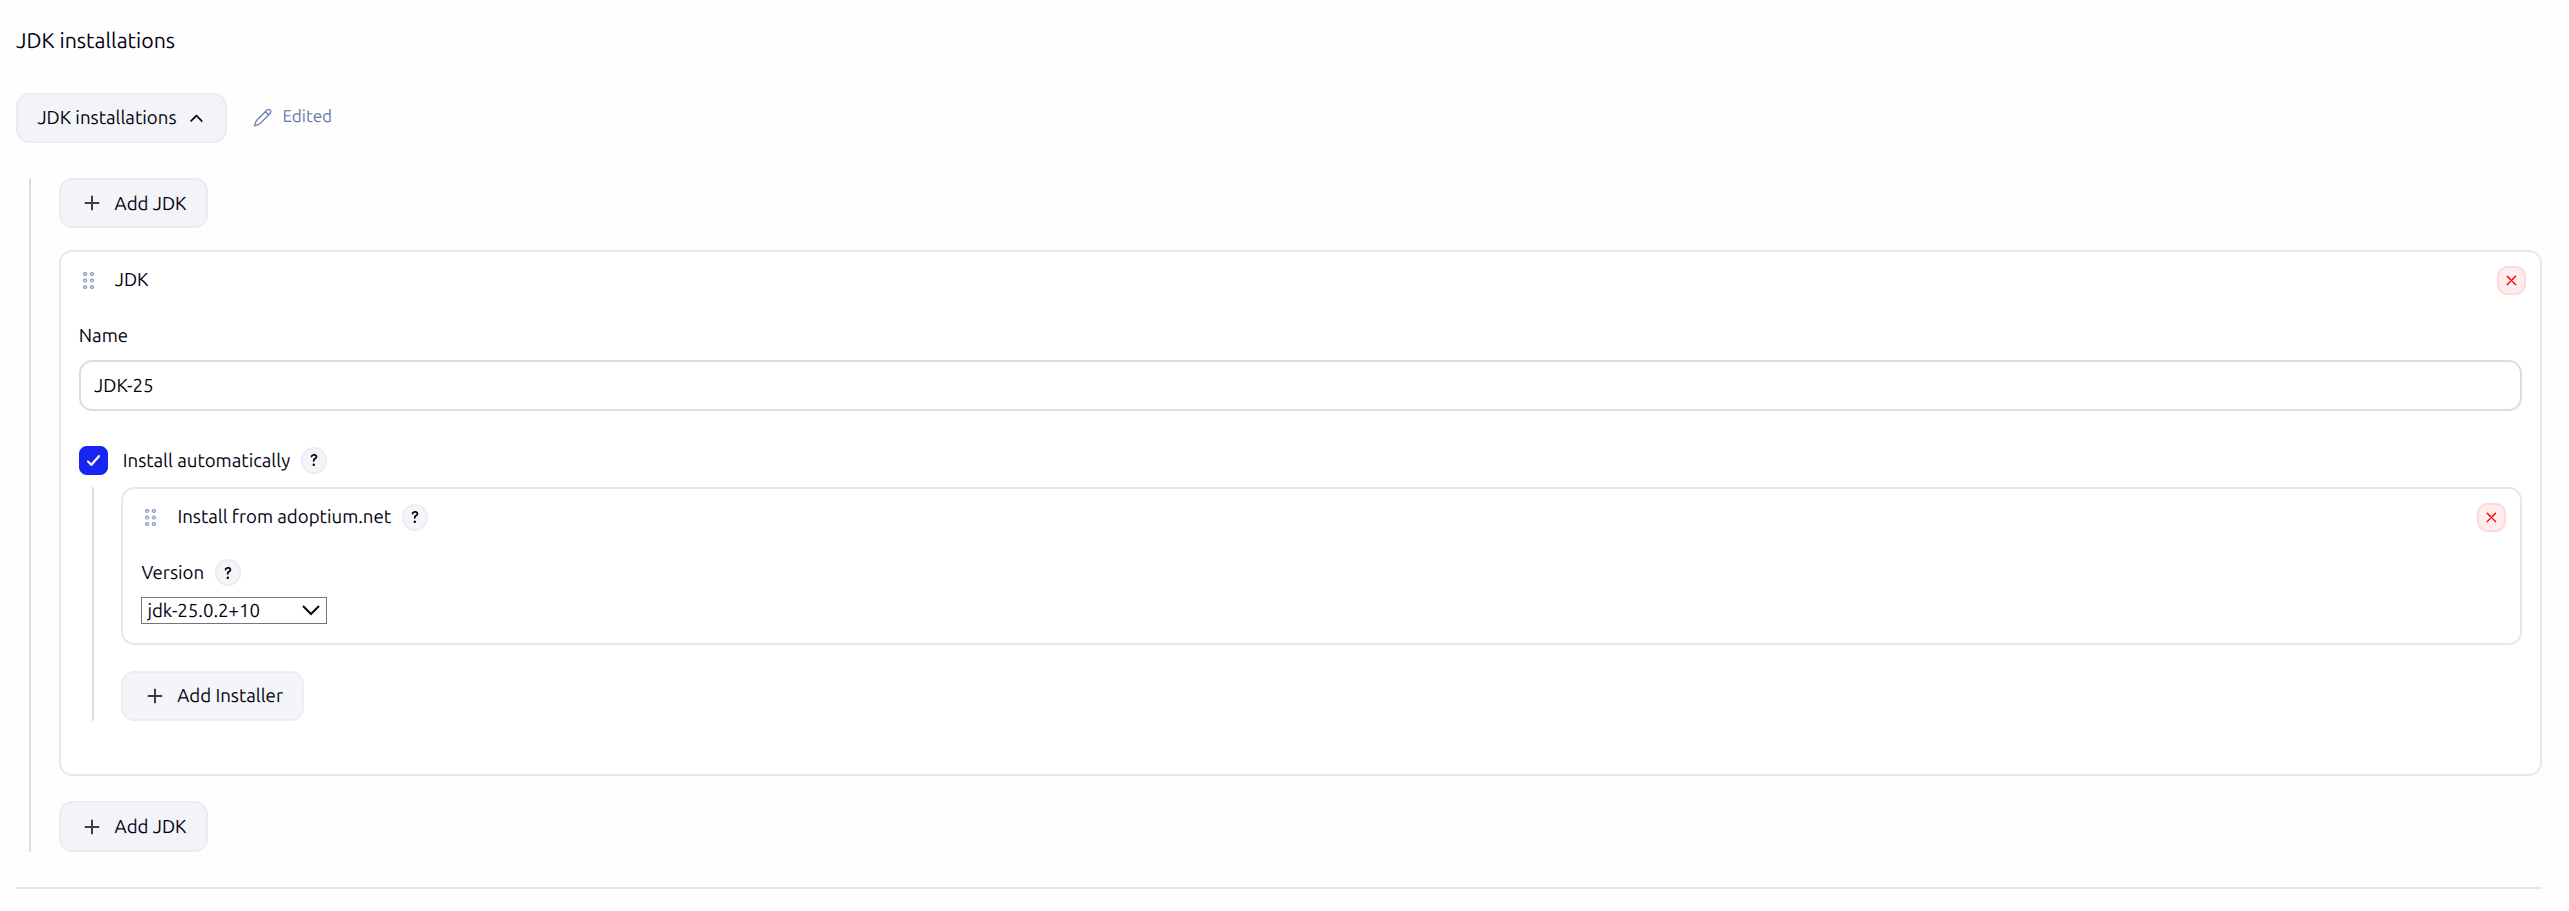
\includegraphics[width=0.9\textwidth]{img/06-jenkins-tools-jdk.png}
    \caption{Cấu hình JDK-25 trong Jenkins Global Tool Configuration}
\end{figure}

\begin{figure}[H]
    \centering
    % CHỈ DẪN ẢNH: Thả ảnh 07-jenkins-tools-maven.png vào thư mục img/
    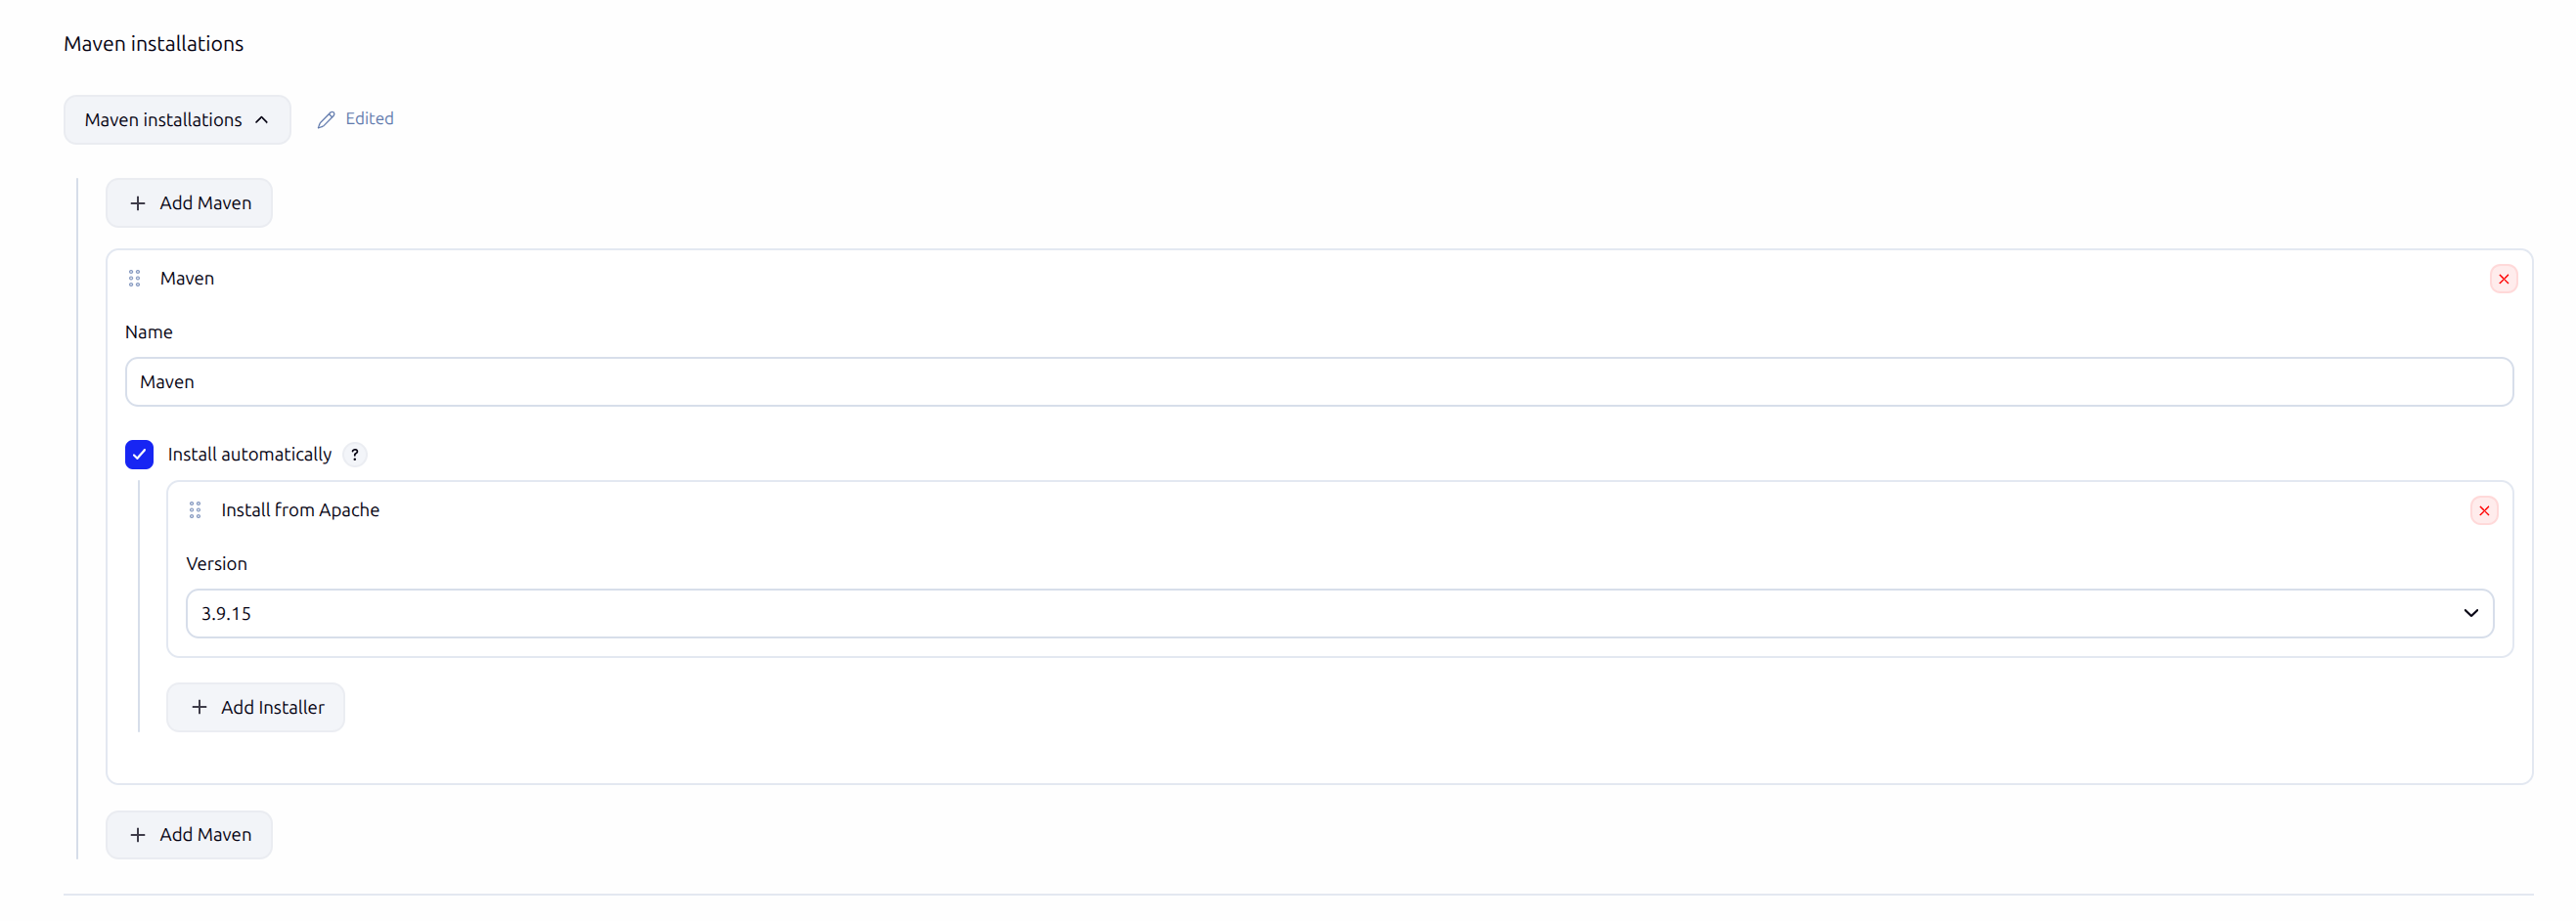
\includegraphics[width=0.9\textwidth]{img/07-jenkins-tools-maven.png}
    \caption{Cấu hình Maven trong Jenkins Global Tool Configuration}
\end{figure}

\subsection{Cấu hình Credentials}
Các credentials được lưu trong Jenkins Credentials Store:
\begin{table}[H]
\centering
\caption{Jenkins Credentials}
\begin{tabular}{|l|l|l|}
\hline
\textbf{ID} & \textbf{Loại} & \textbf{Mục đích} \\
\hline
\texttt{sonarqube-token} & Secret text & Xác thực SonarQube API \\
\hline
\texttt{snyk-token} & Secret text & Xác thực Snyk CLI \\
\hline
\end{tabular}
\end{table}

\begin{figure}[H]
    \centering
    % CHỈ DẪN ẢNH: Thả ảnh 08-jenkins-credentials-ids.png vào thư mục img/
    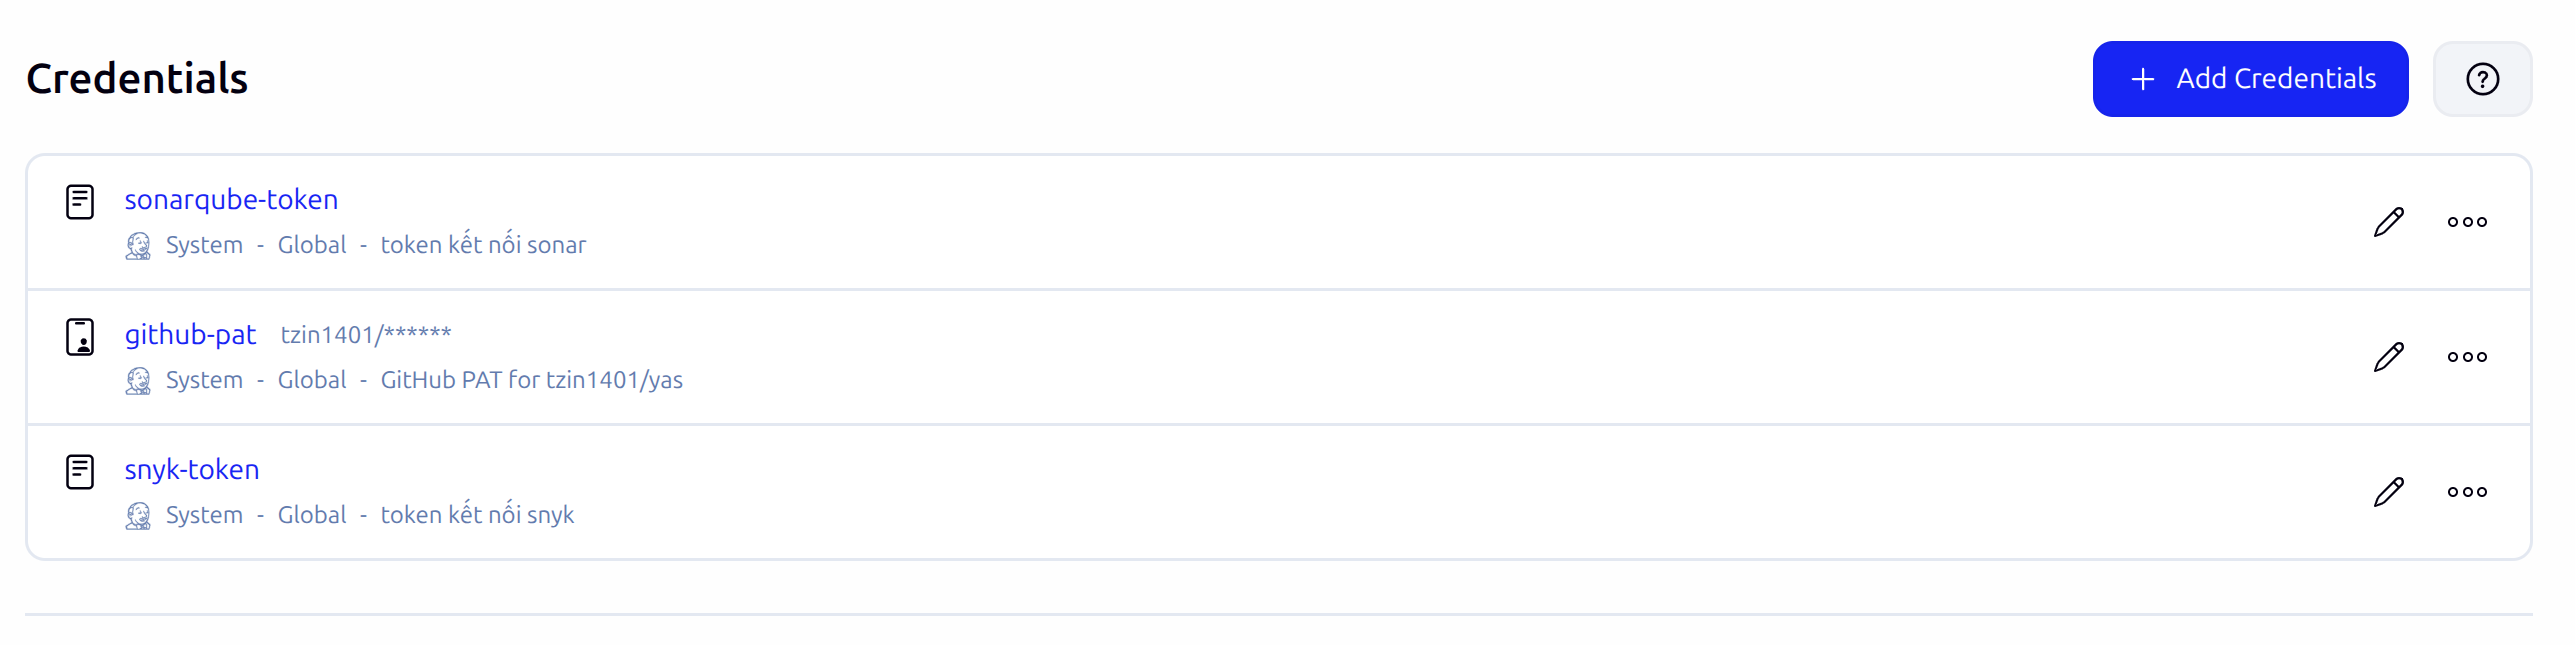
\includegraphics[width=0.9\textwidth]{img/08-jenkins-credentials-ids.png}
    \caption{Danh sách ID Credentials đã được lưu trên Jenkins}
\end{figure}

\subsection{Cấu hình Distributed Build Nodes (Agents)}
Để thực thi các tác vụ build và test một cách phân tán, nhóm đã đăng ký 3 Agent vào hệ thống Jenkins Master:
\begin{itemize}[noitemsep]
    \item \textbf{Agent-Tri}: Agent phụ trách xử lý và thực thi các build job.
    \item \textbf{Agent-QVinh}: Agent phụ trách xử lý và thực thi các build job.
    \item \textbf{Agent-TVinh}: Agent phụ trách xử lý và thực thi các build job.
\end{itemize}

\begin{figure}[H]
    \centering
    % CHỈ DẪN ẢNH: Thả ảnh 08c-jenkins-agent-nodes.png vào thư mục img/
    % Nội dung: Màn hình Manage Jenkins -> Nodes hiển thị cả 3 agent online
    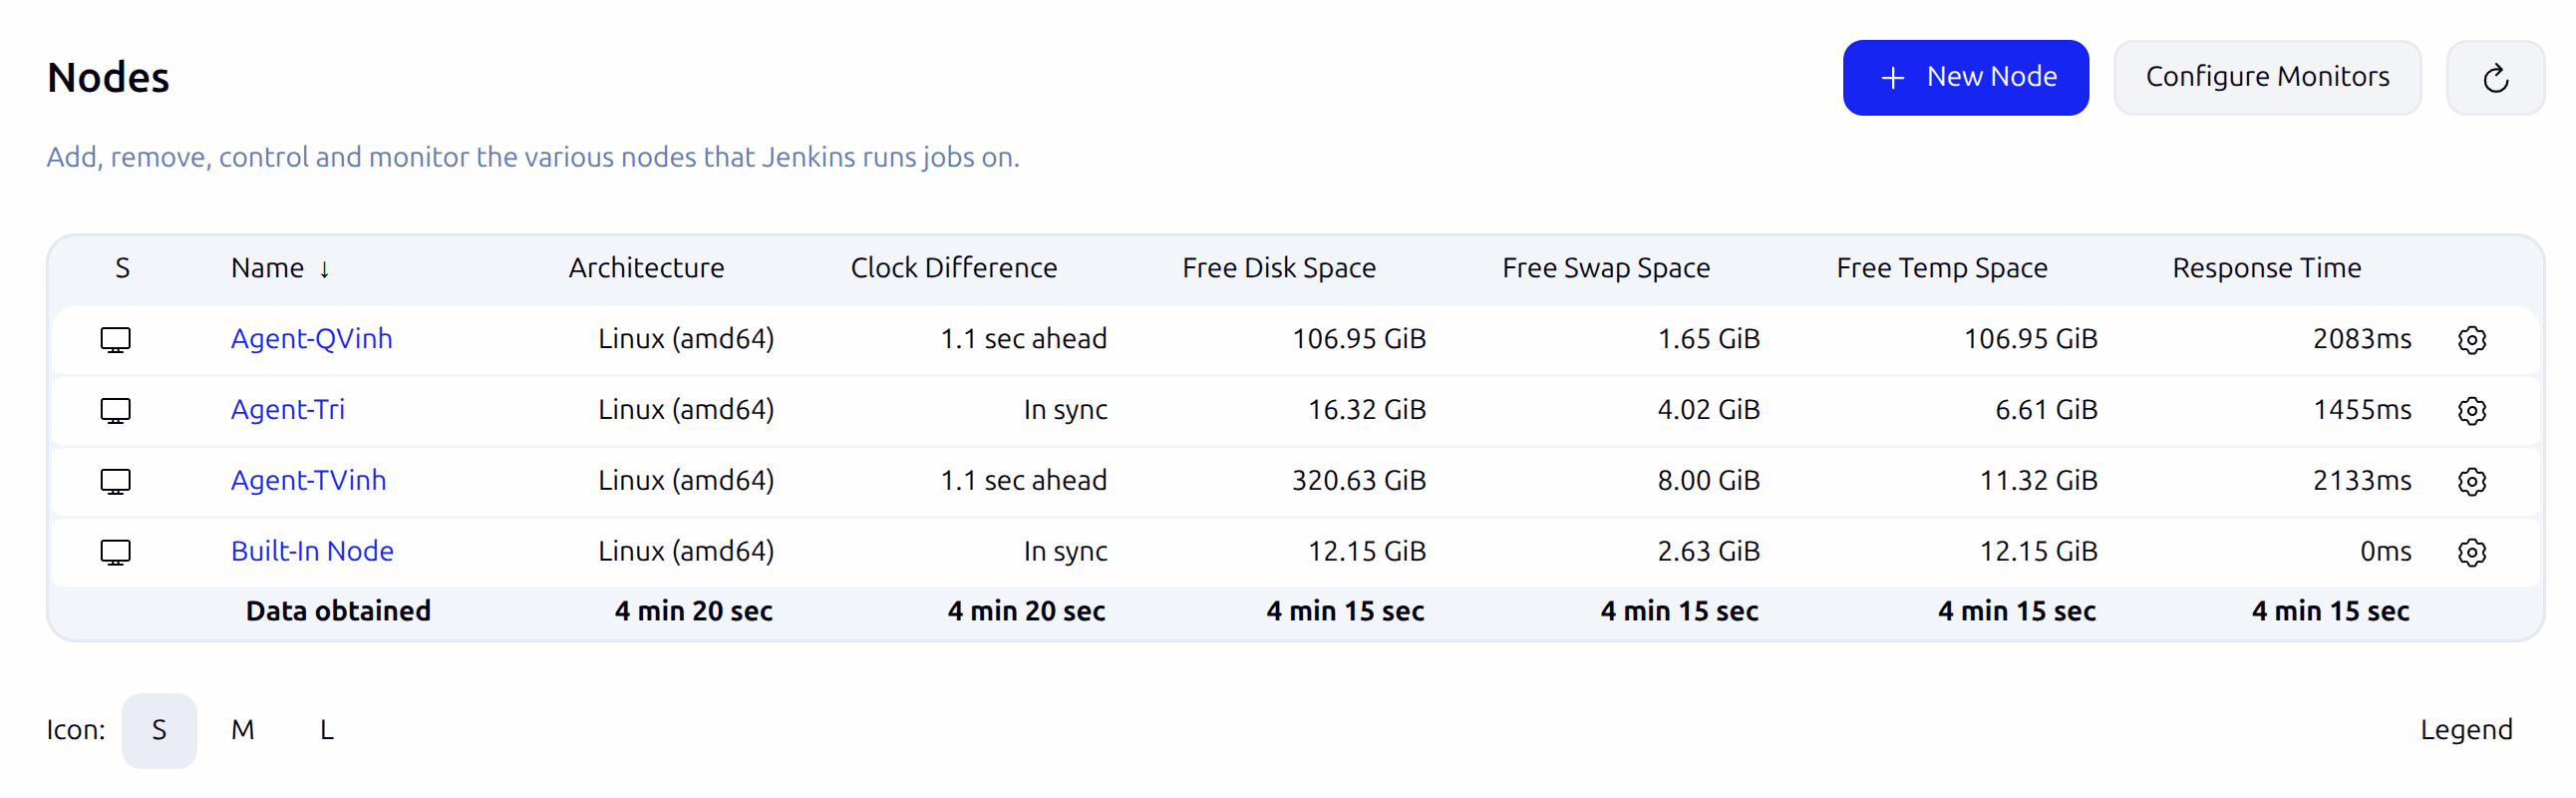
\includegraphics[width=0.9\textwidth]{img/08c-jenkins-agent-nodes.png}
    \caption{Danh sách các Nodes/Agents đã kết nối thành công với Jenkins Master}
\end{figure}

\subsubsection{Thiết lập Jenkins Agent (Node) và Cách kết nối}
Trong mô hình Distributed Build, Jenkins Master chỉ điều khiển, còn Agent (Node) là nơi thực sự chạy code.

\textbf{1.1 Các bước tạo Node trên giao diện Jenkins}:
\begin{enumerate}[noitemsep]
    \item Truy cập \textbf{Manage Jenkins} $\rightarrow$ \textbf{Nodes} $\rightarrow$ \textbf{New Node}.
    \item Đặt tên (vd: \texttt{Agent-QVinh}), chọn \textbf{Permanent Agent}.
    \item \textbf{Remote root directory}: Thư mục làm việc trên máy Agent (vd: \texttt{/home/ubuntu/jenkins-agent}).
    \item \textbf{Launch method}: Chọn \textbf{Launch agent by connecting it to the controller} (kết nối từ máy Agent đến Master qua JNLP).
\end{enumerate}

\textbf{1.2 Cách kết nối từ máy Agent đến Node (Master)}:
Sau khi nhấn Save, Jenkins sẽ cung cấp một đoạn mã lệnh. Nhóm tiến hành SSH vào máy Agent và thực hiện:
\begin{enumerate}[noitemsep]
    \item Tải file \texttt{agent.jar}:
\begin{lstlisting}[language=bash]
curl -sO http://<IP-Jenkins-Master>:8080/jnlpJars/agent.jar
\end{lstlisting}
    \item Chạy lệnh kết nối:
\begin{lstlisting}[language=bash]
java -jar agent.jar -url http://<IP-Jenkins-Master>:8080/ -secret <SECRET_KEY> -name "Agent-QVinh" -workDir "/home/ubuntu/jenkins-agent"
\end{lstlisting}
    \item \textit{Lưu ý}: Để Agent tự khởi chạy lại khi khởi động máy, nhóm cấu hình lệnh này thành một Systemd Service trên Linux.
\end{enumerate}

\subsubsection{Cài đặt môi trường thực thi (Tooling) trên Agent}
Để chạy được toàn bộ Pipeline ``yas'', các máy Agent (Node) được cài đặt các công cụ sau:
\begin{itemize}[noitemsep]
    \item \textbf{Docker Engine \& Docker Compose}: Cài đặt để thực hiện Stage Build Image và quét Snyk Container. Đồng thời, chạy lệnh \texttt{sudo usermod -aG docker jenkins} và khởi động lại Agent để user Jenkins có quyền thực thi lệnh Docker.
    \item \textbf{Java Development Kit (JDK)}: Cài đặt phiên bản khớp với dự án (ví dụ JDK 25) để thực thi file \texttt{agent.jar} và chạy Maven.
    \item \textbf{Apache Maven}: Cài đặt để chạy lệnh \texttt{mvn test}, \texttt{mvn dependency:tree} và các lệnh kiểm tra coverage.
    \item \textbf{Git}: Cài đặt để Agent có thể thực hiện Stage Checkout code từ GitHub.
\end{itemize}

\subsubsection{Cấu hình Snyk Auth trên Terminal của Agent}
Trong môi trường CI/CD, việc xác thực Agent bằng Token là tối ưu nhất.

\begin{enumerate}[noitemsep]
    \item \textbf{Cài đặt Snyk CLI}: Agent cài đặt Snyk thông qua lệnh \texttt{npm install -g snyk}.
    \item \textbf{Xác thực bằng Token}: Trên Terminal của Agent, chạy lệnh: \texttt{snyk auth <YOUR\_SNYK\_API\_TOKEN>} hoặc gán biến môi trường \texttt{SNYK\_TOKEN} để Snyk tự động nhận diện.
\end{enumerate}

\begin{figure}[H]
    \centering
    % CHỈ DẪN ẢNH: Thả ảnh 09b-snyk-auth-agent.png vào thư mục img/
    % Nội dung: Chụp màn hình terminal gõ lệnh auth và hiển thị thành công "Your account has been successfully authenticated"
    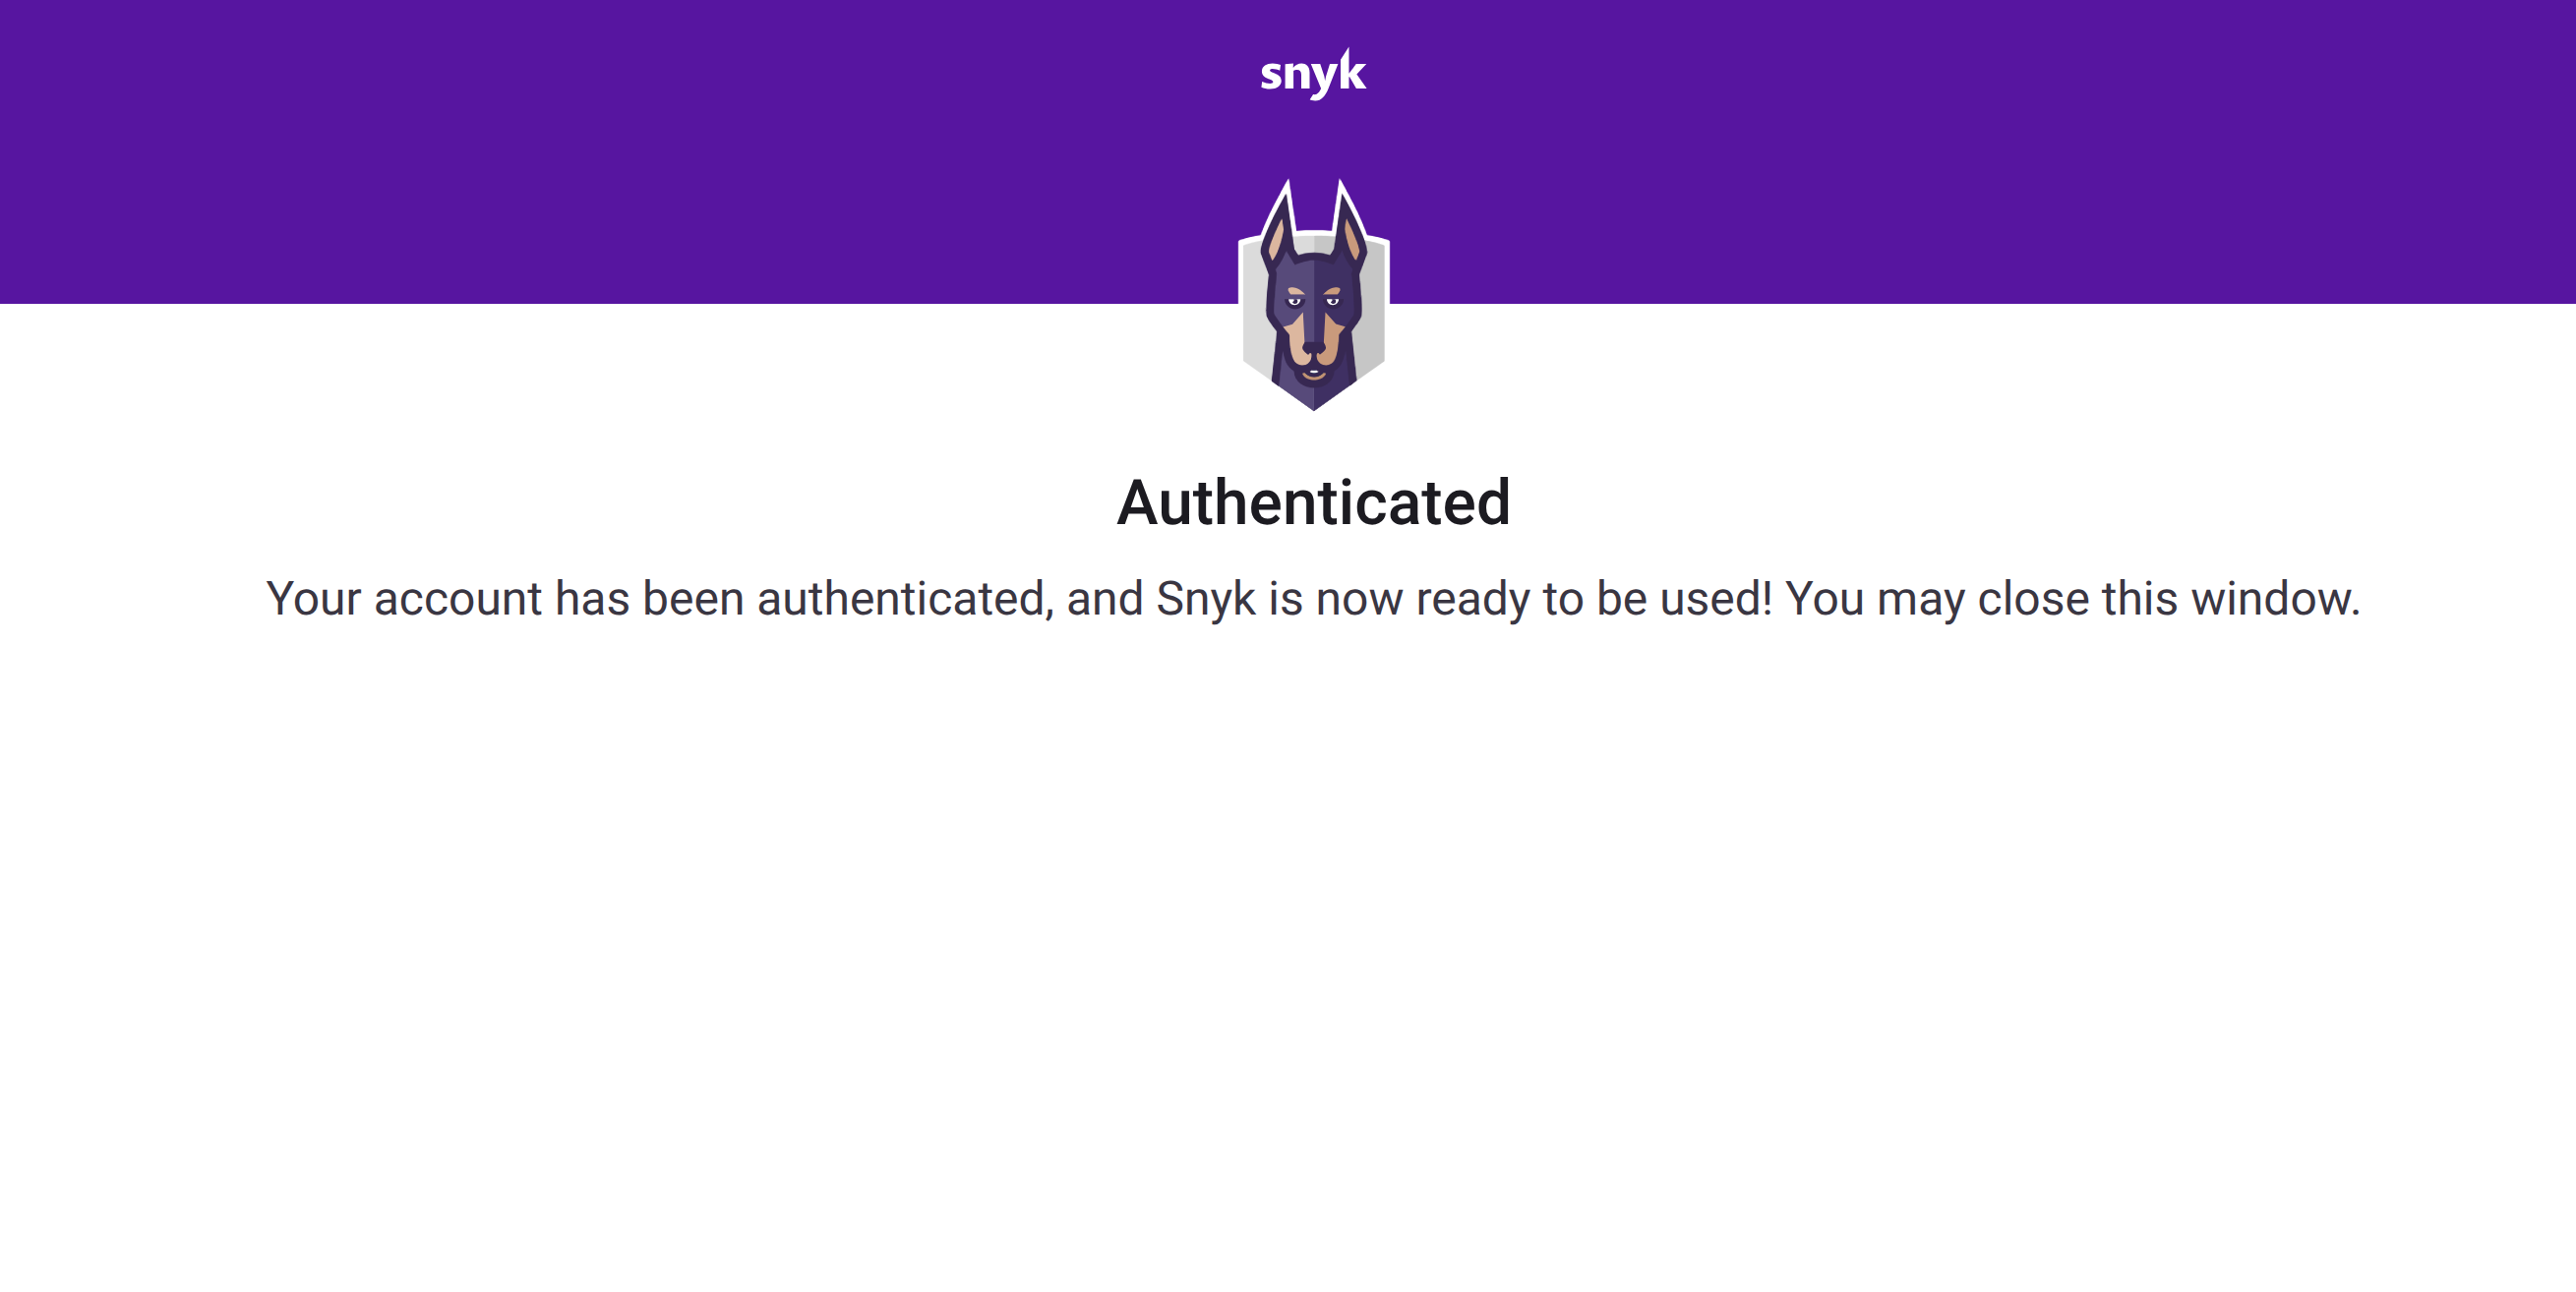
\includegraphics[width=0.9\textwidth]{img/09b-snyk-auth-agent.png}
    \caption{Xác thực tài khoản Snyk thành công trên Agent}
\end{figure}

\subsection{Cấu hình hiển thị Biểu đồ và Thống kê (Plugins)}
Để Jenkins hiển thị được các tab báo cáo và biểu đồ từ kết quả quét, nhóm đã cấu hình các Plugin sau trên Master:

\begin{itemize}
    \item \textbf{JaCoCo Plugin}: Sau khi chạy \texttt{mvn jacoco:report}, plugin này đọc file \texttt{.exec} trong thư mục target để hiển thị biểu đồ Coverage Trend ngay tại trang chủ của Job.
\end{itemize}

\begin{figure}[H]
    \centering
    % CHỈ DẪN ẢNH: Thả ảnh 10b-jenkins-jacoco-coverage-trend.png vào thư mục img/
    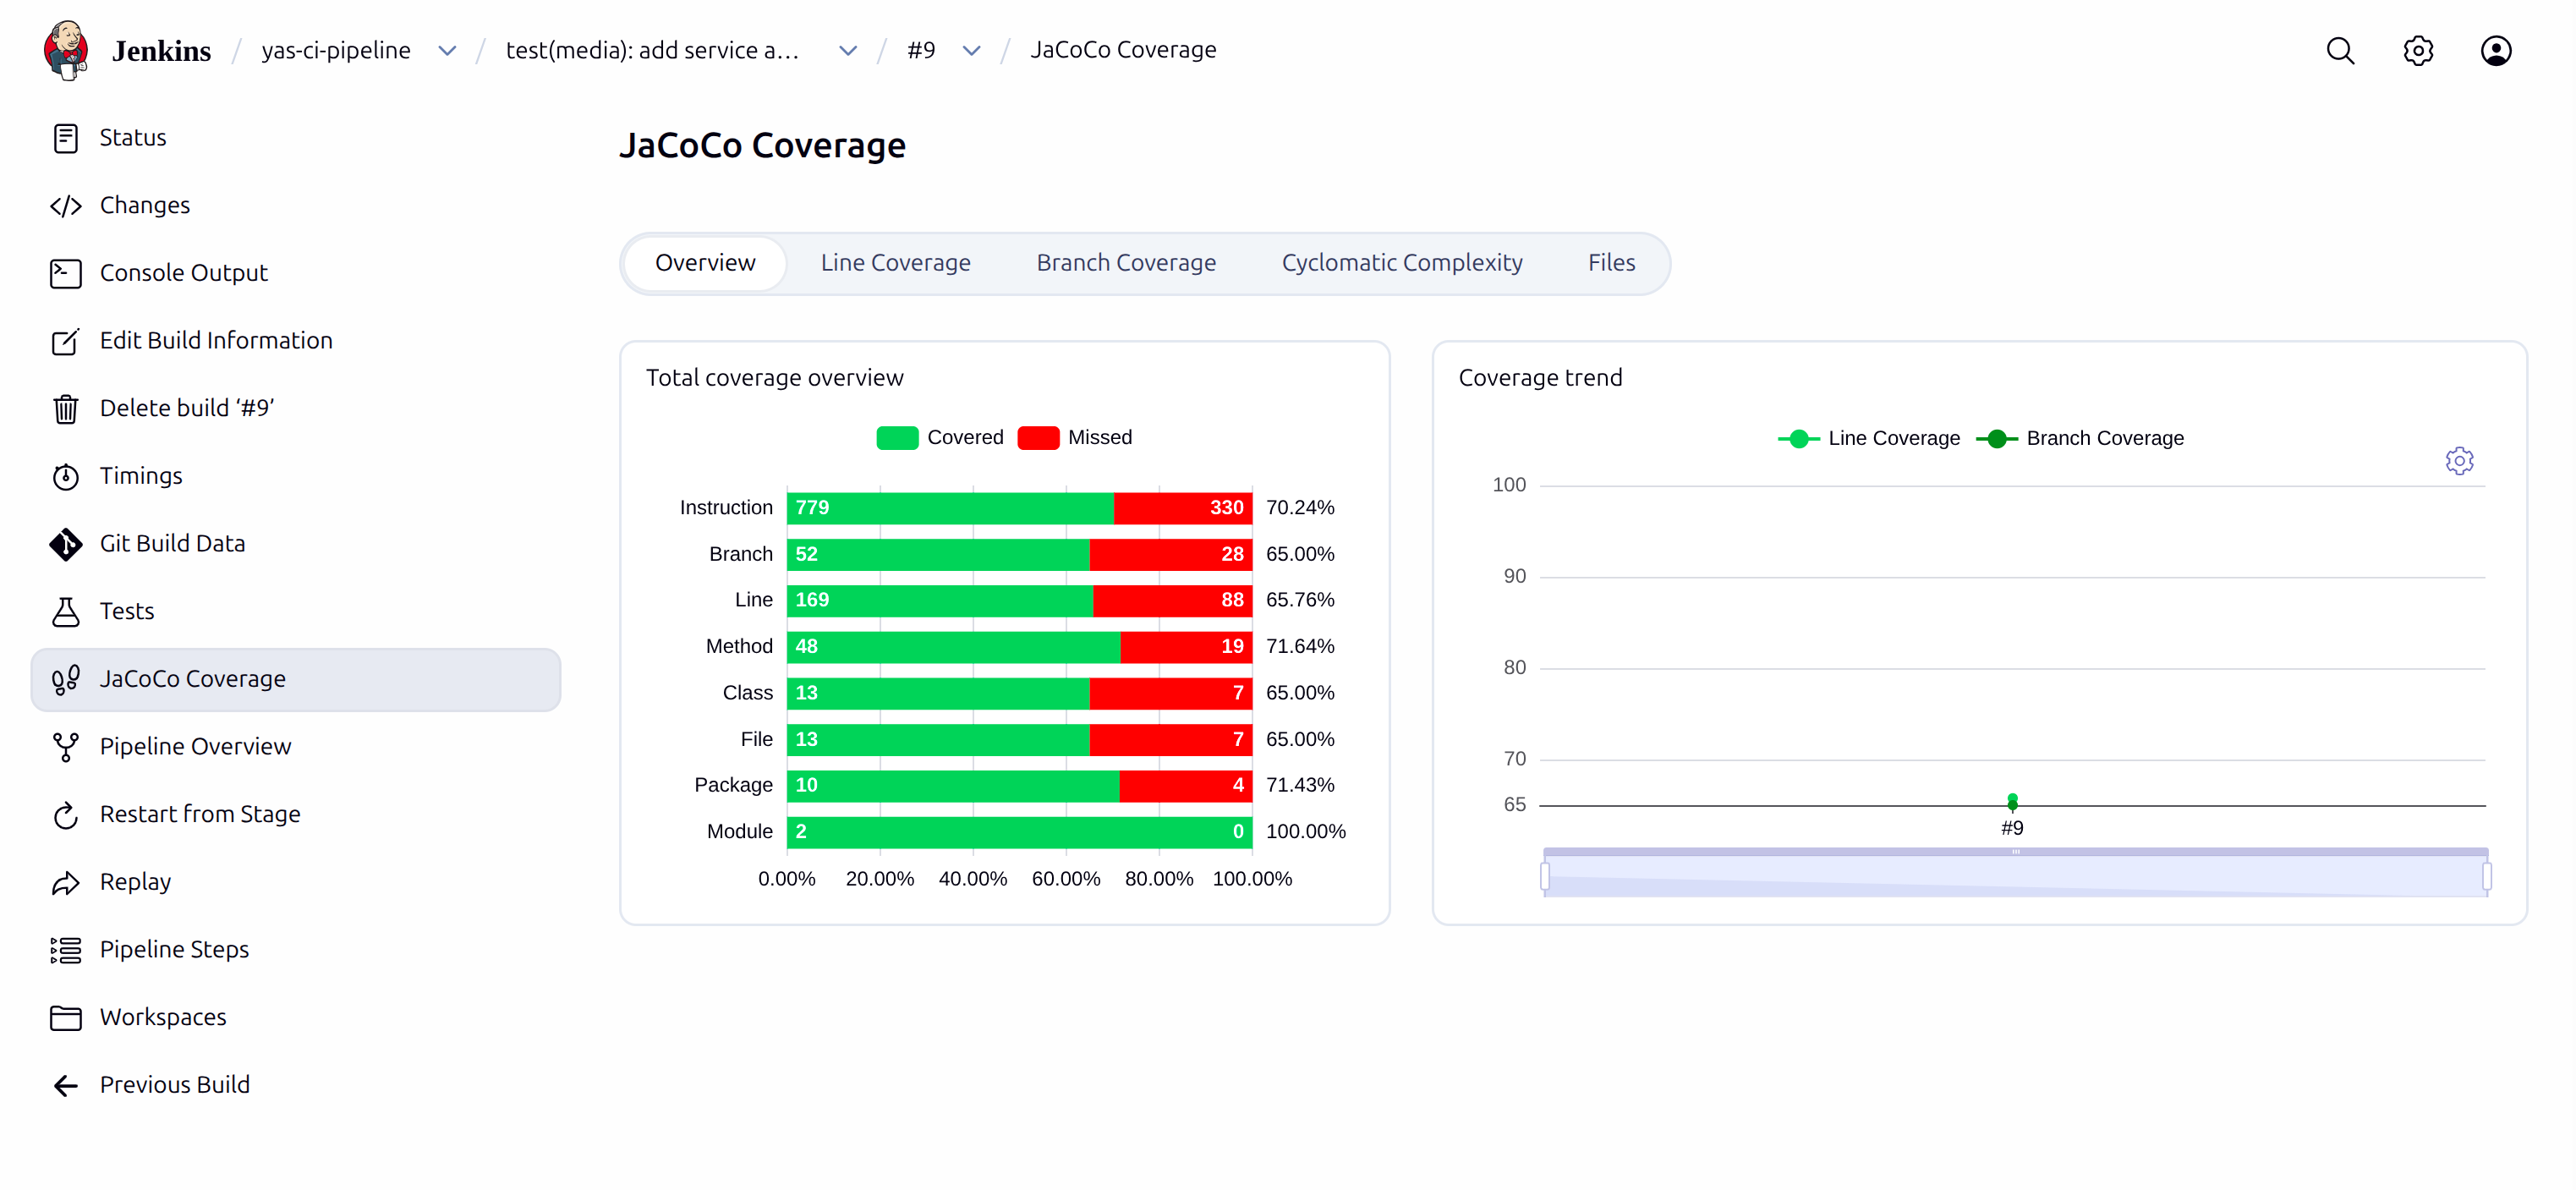
\includegraphics[width=0.9\textwidth]{img/10b-jenkins-jacoco-coverage-trend.png}
    \caption{Biểu đồ Coverage Trend hiển thị thông qua JaCoCo Plugin}
\end{figure}

\begin{itemize}
    \item \textbf{SonarQube Scanner Plugin}: Cấu hình Webhook trỏ về \texttt{/sonarqube-webhook/} để hiển thị trạng thái Quality Gate (Passed/Failed) trực tiếp trên Pipeline.
\end{itemize}

\begin{figure}[H]
    \centering
    % CHỈ DẪN ẢNH: Thả ảnh 08b-jenkins-system-sonarqube-server.png vào thư mục img/
    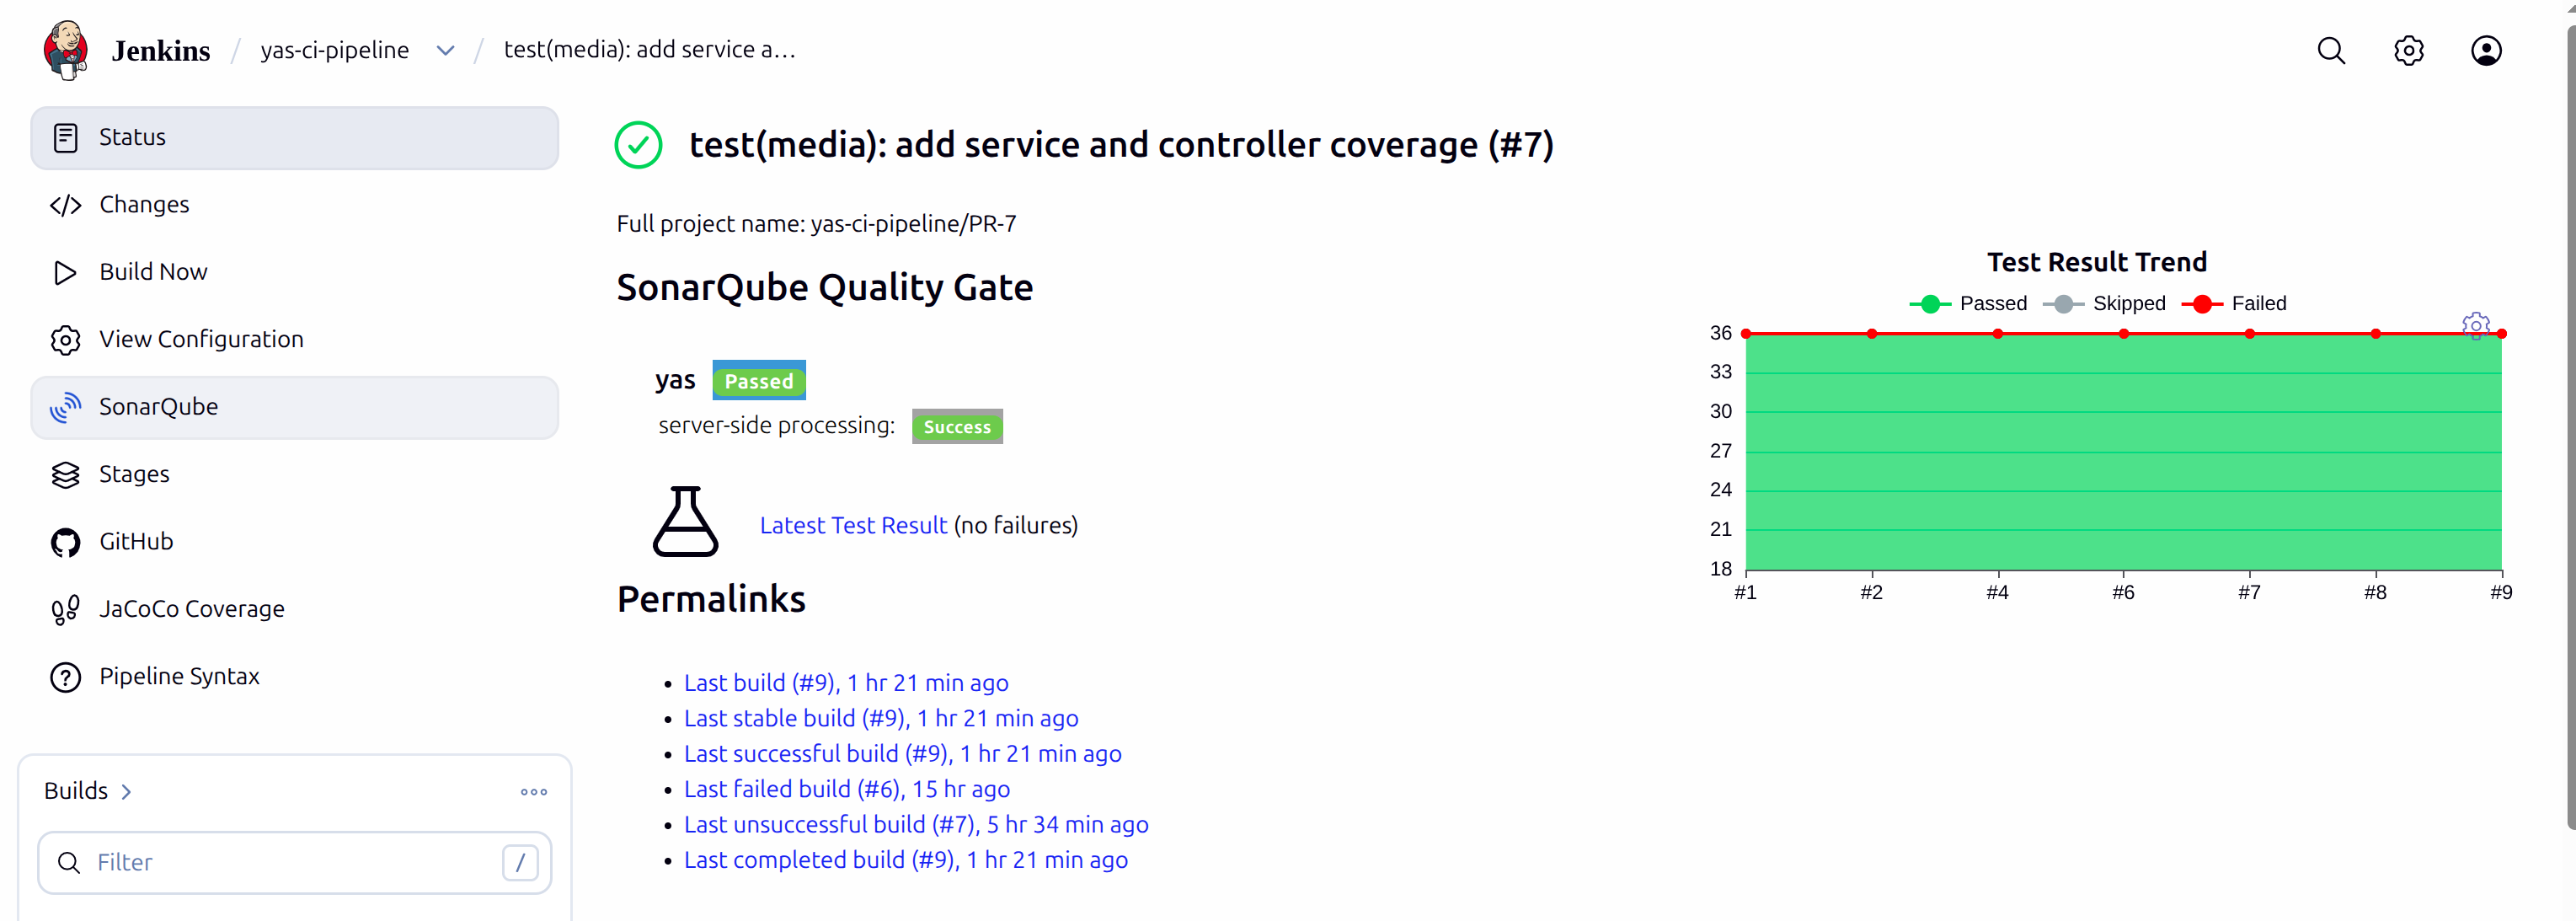
\includegraphics[width=0.9\textwidth]{img/08b-jenkins-system-sonarqube-server.png}
    \caption{Thống kê của SonarQube}
\end{figure}

\begin{itemize}
    \item \textbf{Snyk Security Plugin}: Cho phép xem chi tiết các lỗ hổng (Vulnerabilities) theo mức độ nghiêm trọng (High, Medium, Low) ngay trong giao diện Jenkins.
\end{itemize}

\subsection{Tạo Multibranch Pipeline Job}
Nhóm tạo job \texttt{yas-ci-pipeline} với loại \textbf{Multibranch Pipeline}:

\begin{enumerate}[noitemsep]
    \item \textbf{Branch Sources}: GitHub repository \texttt{tzin1401/yas}
    \item \textbf{Discover branches}: Strategy ``Exclude branches that are also filed as PRs'' --- tránh build trùng lặp khi branch đã có PR
    \item \textbf{Discover pull requests from origin}: Merging the pull request with the current target branch revision
    \item \textbf{Build Configuration}: Jenkinsfile tại root của repository
    \item \textbf{Scan Repository Triggers}: Tự động quét mỗi khi có webhook từ GitHub
\end{enumerate}

\begin{figure}[H]
    \centering
    % CHỈ DẪN ẢNH: Thả ảnh 04-jenkins-config-branch-sources.png vào thư mục img/
    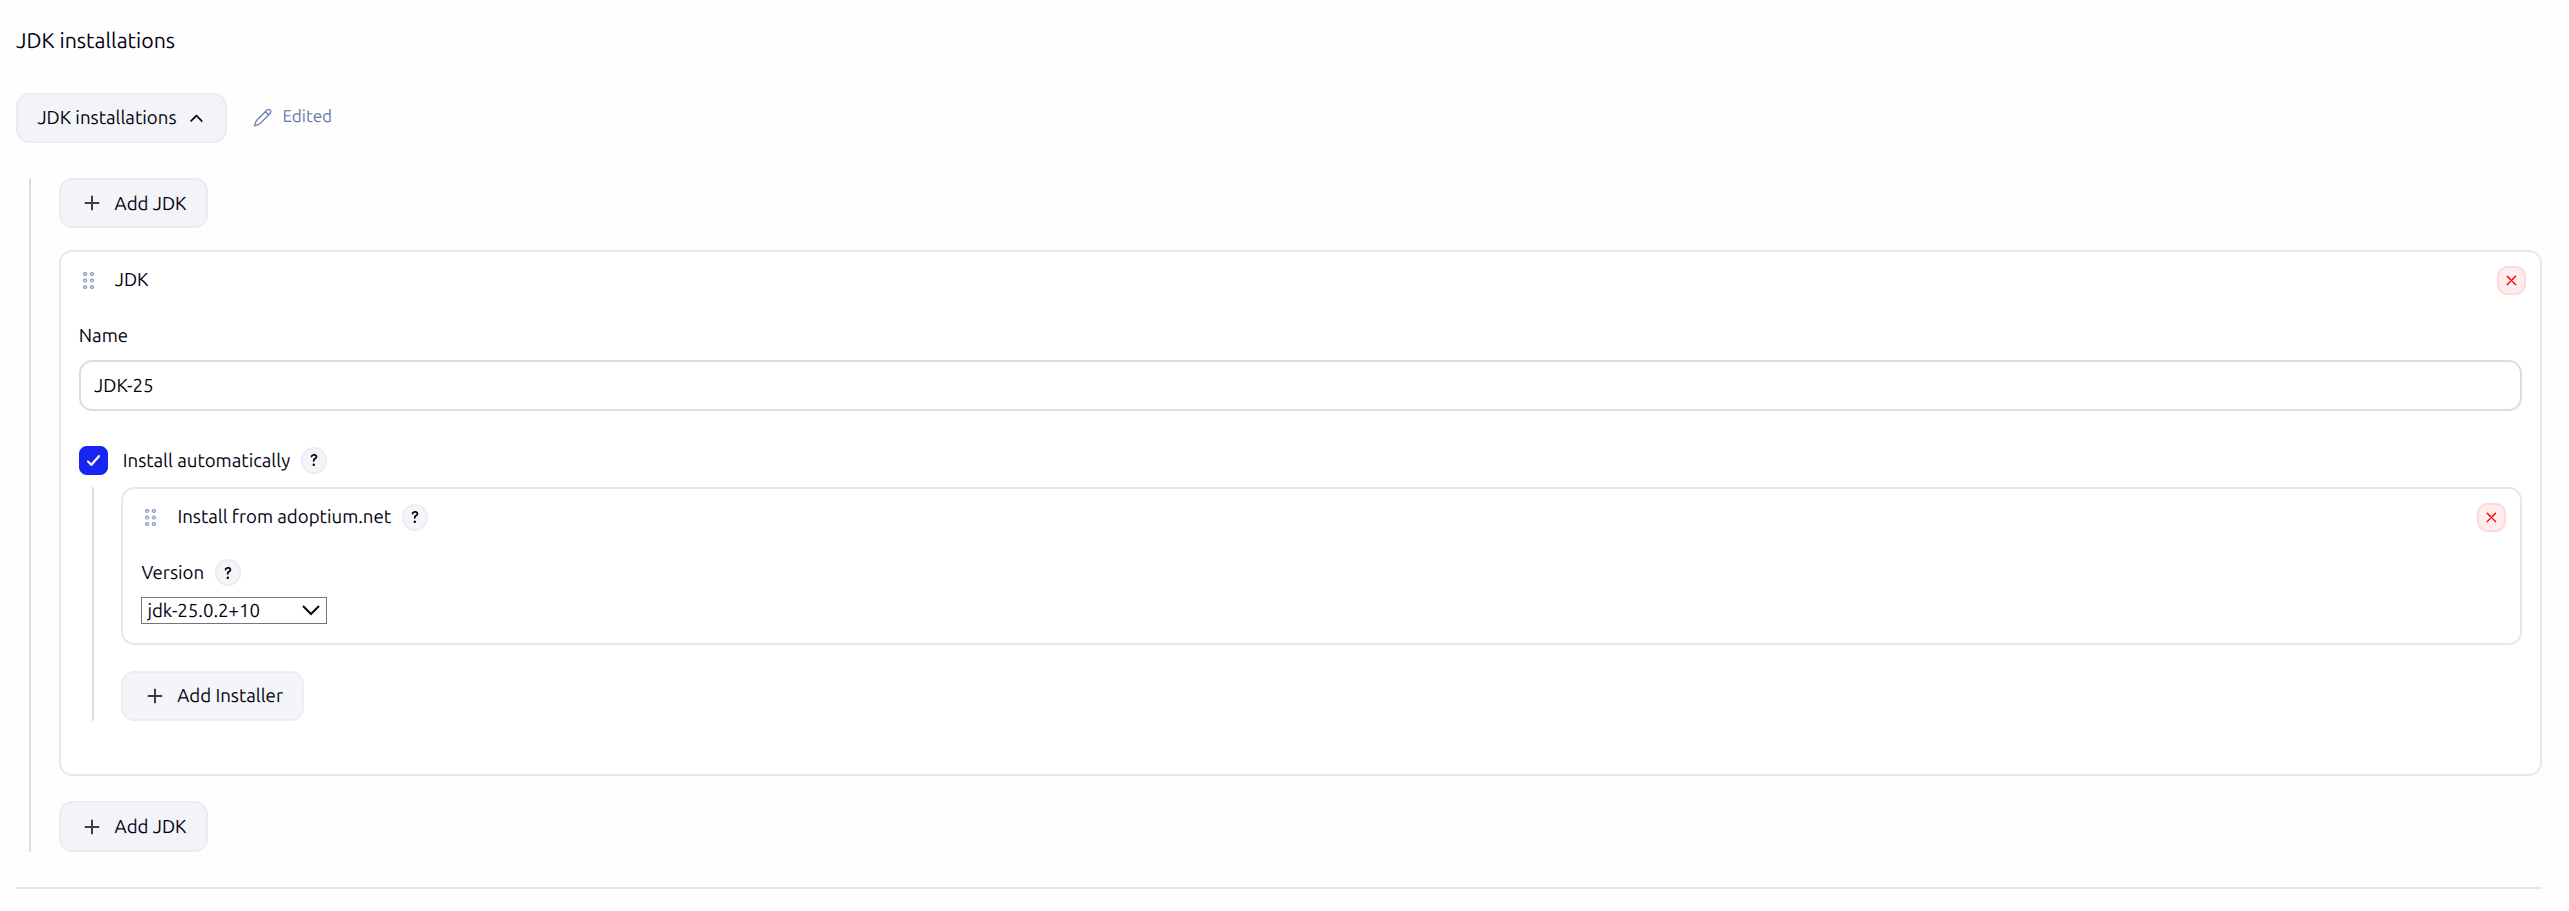
\includegraphics[width=0.9\textwidth]{img/04-jenkins-config-branch-sources.png}
    \caption{Cấu hình Branch Sources trong Multibranch Pipeline Job}
\end{figure}

\begin{figure}[H]
    \centering
    % CHỈ DẪN ẢNH: Thả ảnh 05-jenkins-config-jenkinsfile-path.png vào thư mục img/
    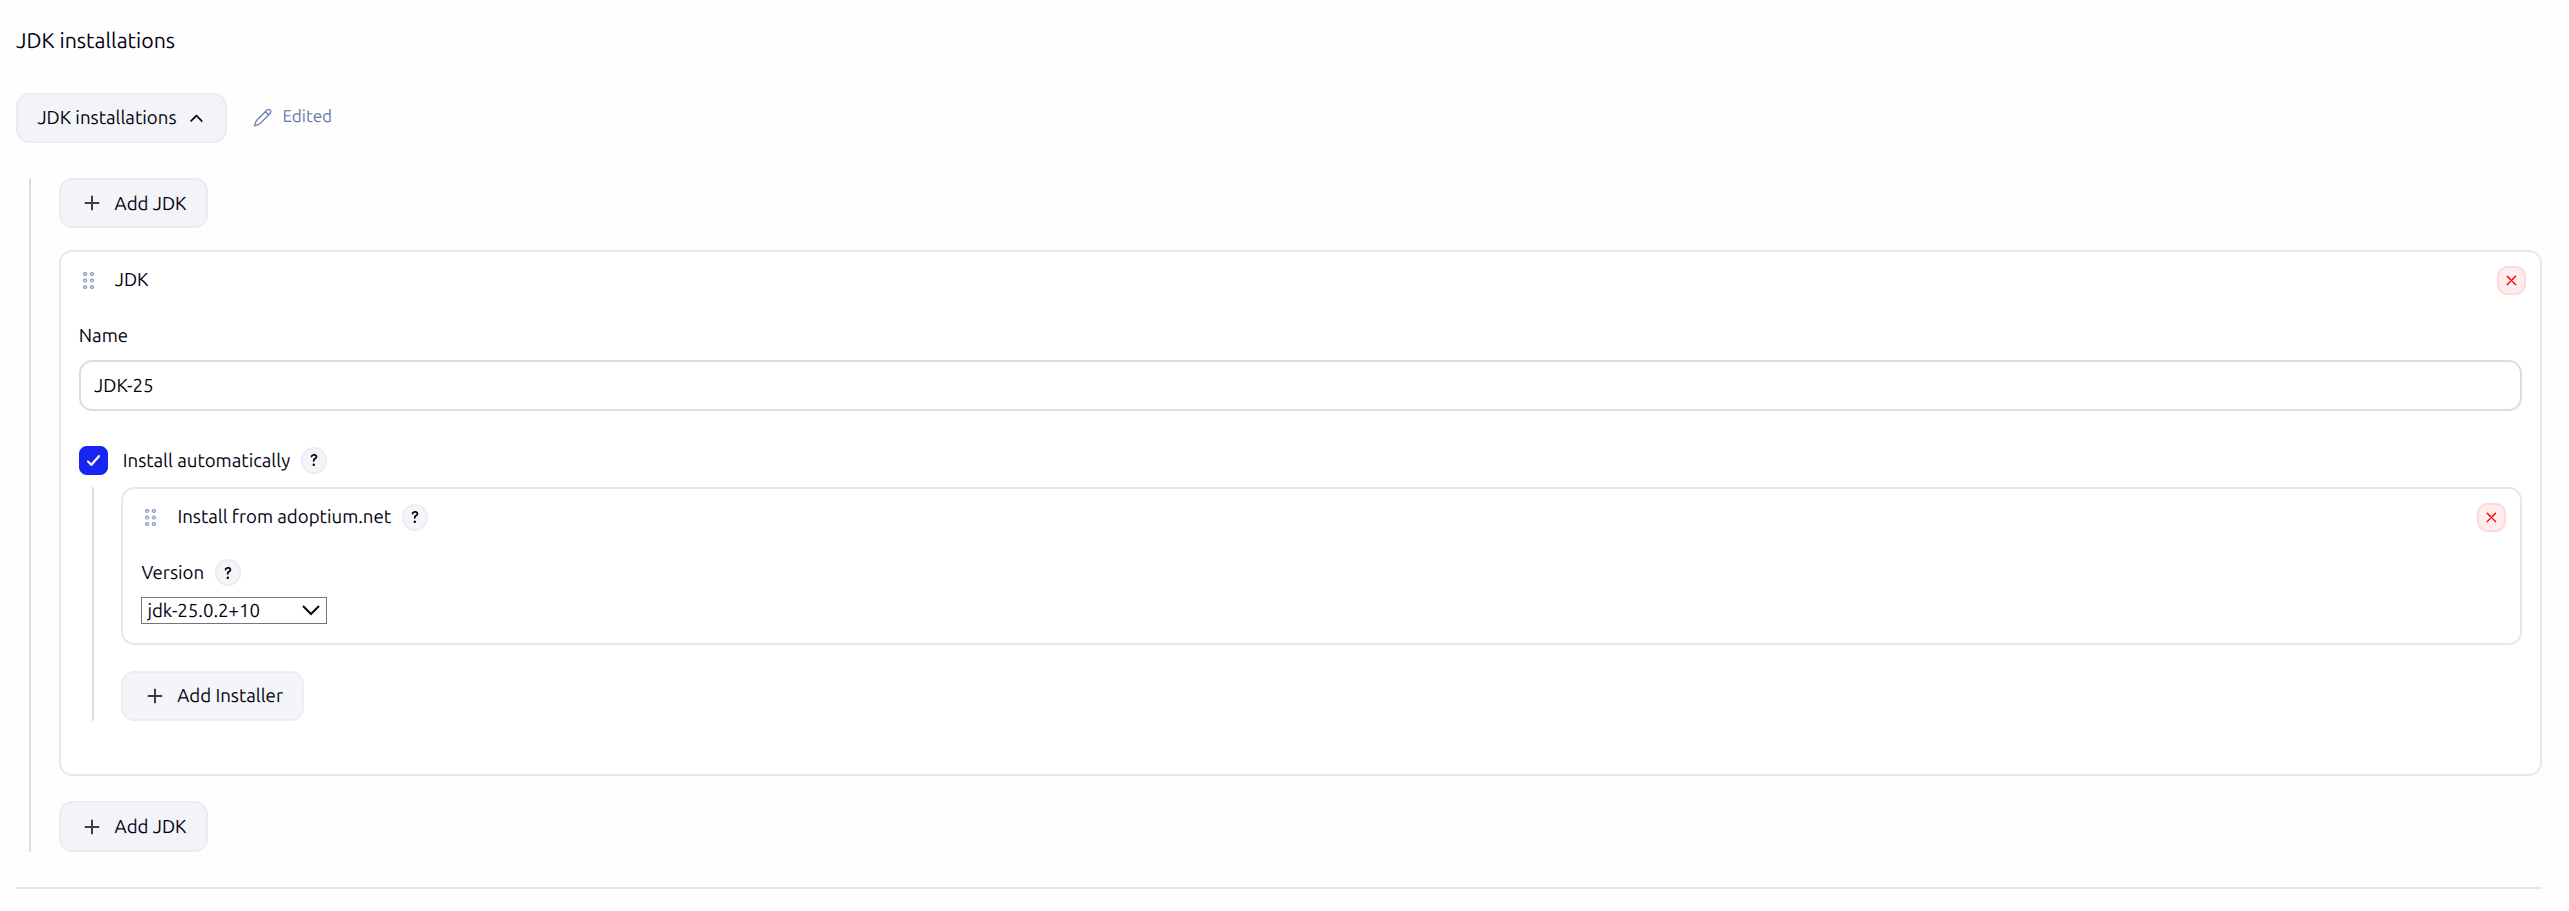
\includegraphics[width=0.9\textwidth]{img/05-jenkins-config-jenkinsfile-path.png}
    \caption{Cấu hình đường dẫn Jenkinsfile trong Multibranch Pipeline Job}
\end{figure}

\subsection{Kết quả: Jenkins tracking branches và PRs}
Sau khi cấu hình, Jenkins tự động phát hiện và tracking:
\begin{itemize}[noitemsep]
    \item \textbf{5 branches}: main, ci/setup-jenkins-pipeline, feature/media-tests, tri/tax-tests, test/ci-path-filter
    \item \textbf{5 pull requests}: PR \#3, \#4, \#5, \#6, \#7
\end{itemize}

\begin{figure}[H]
    \centering
    % CHỈ DẪN ẢNH: Thả ảnh 02-jenkins-multibranch-branches.png vào thư mục img/
    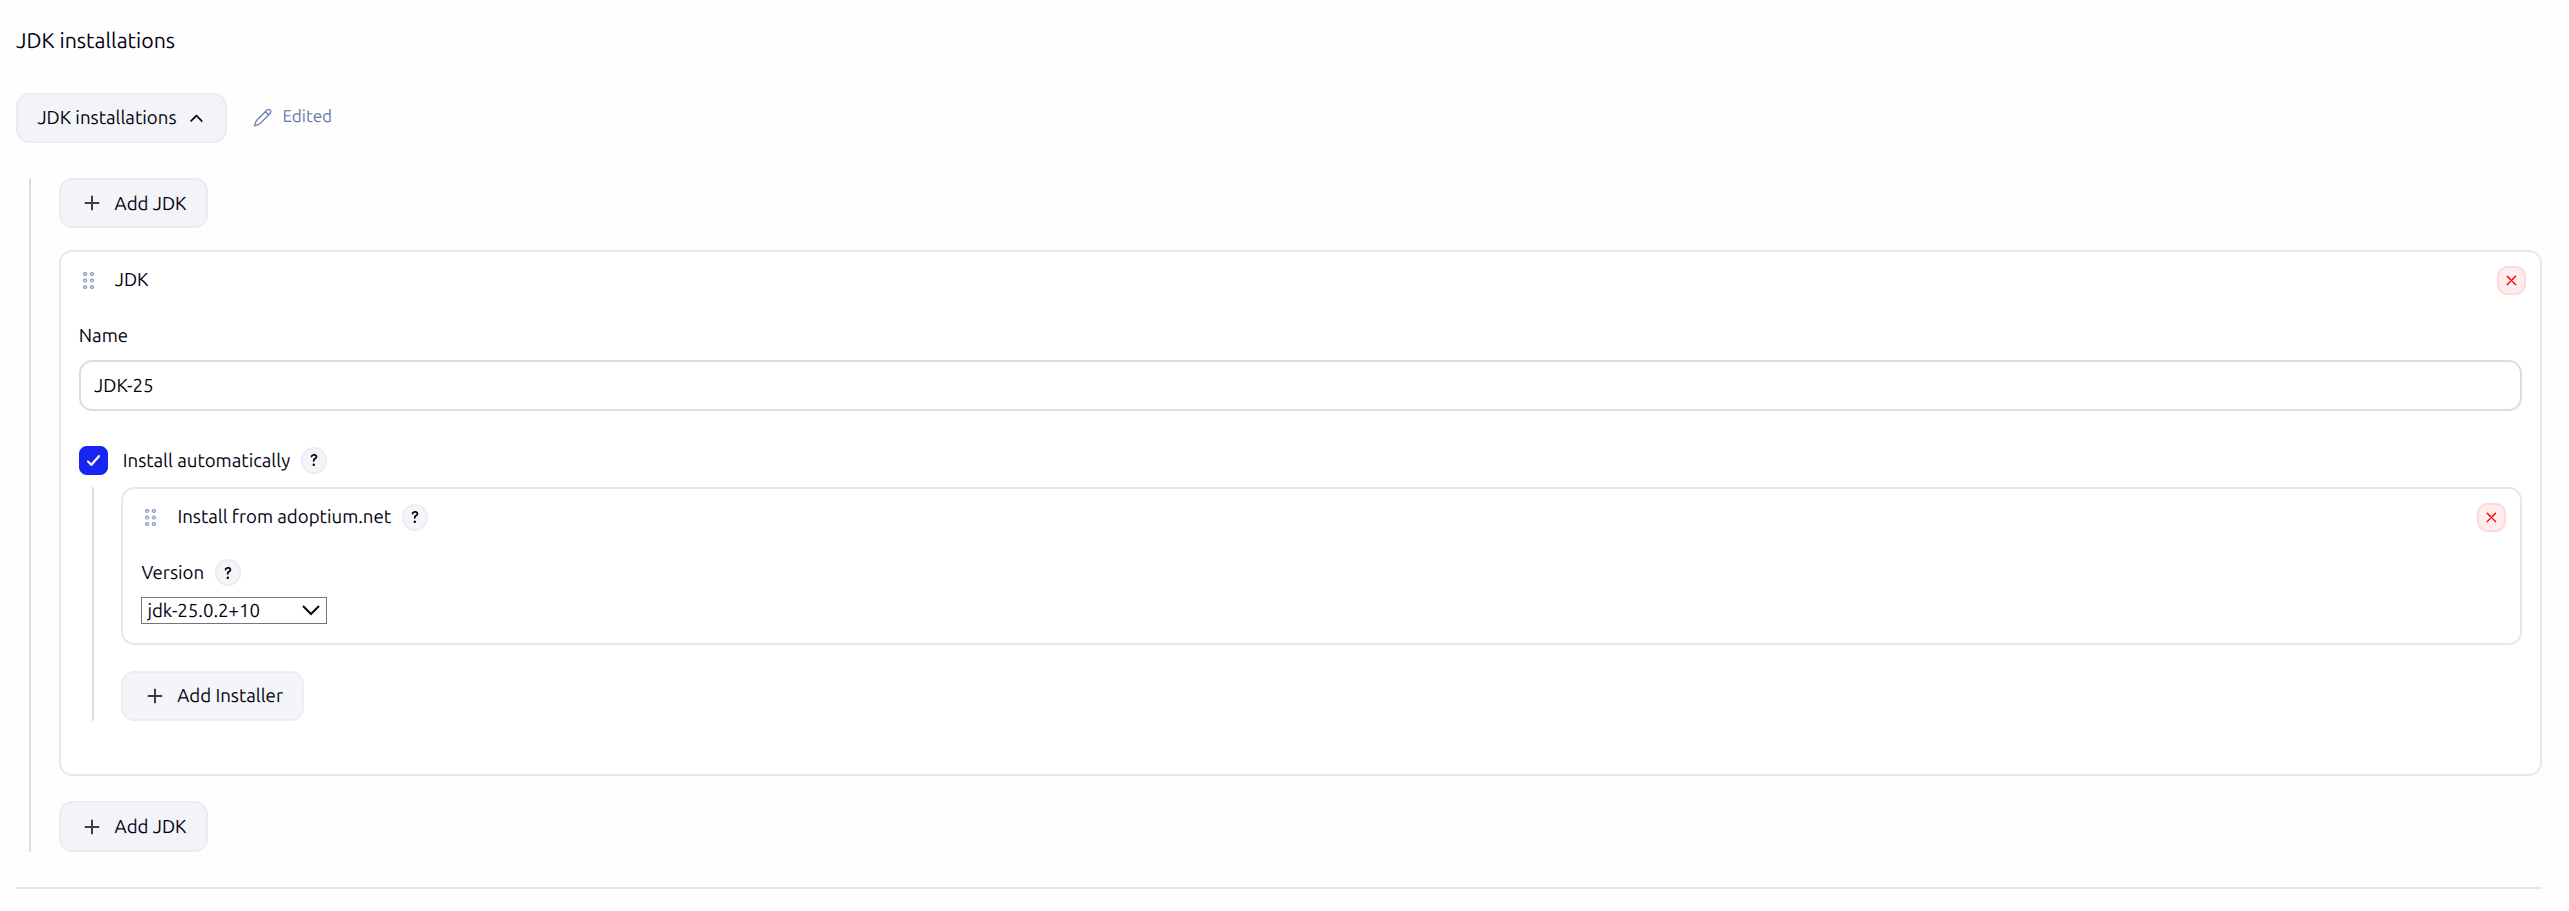
\includegraphics[width=0.9\textwidth]{img/02-jenkins-multibranch-branches.png}
    \caption{Danh sách các nhánh được tự động phát hiện và build}
\end{figure}

\begin{figure}[H]
    \centering
    % CHỈ DẪN ẢNH: Thả ảnh 03-jenkins-multibranch-prs.png vào thư mục img/
    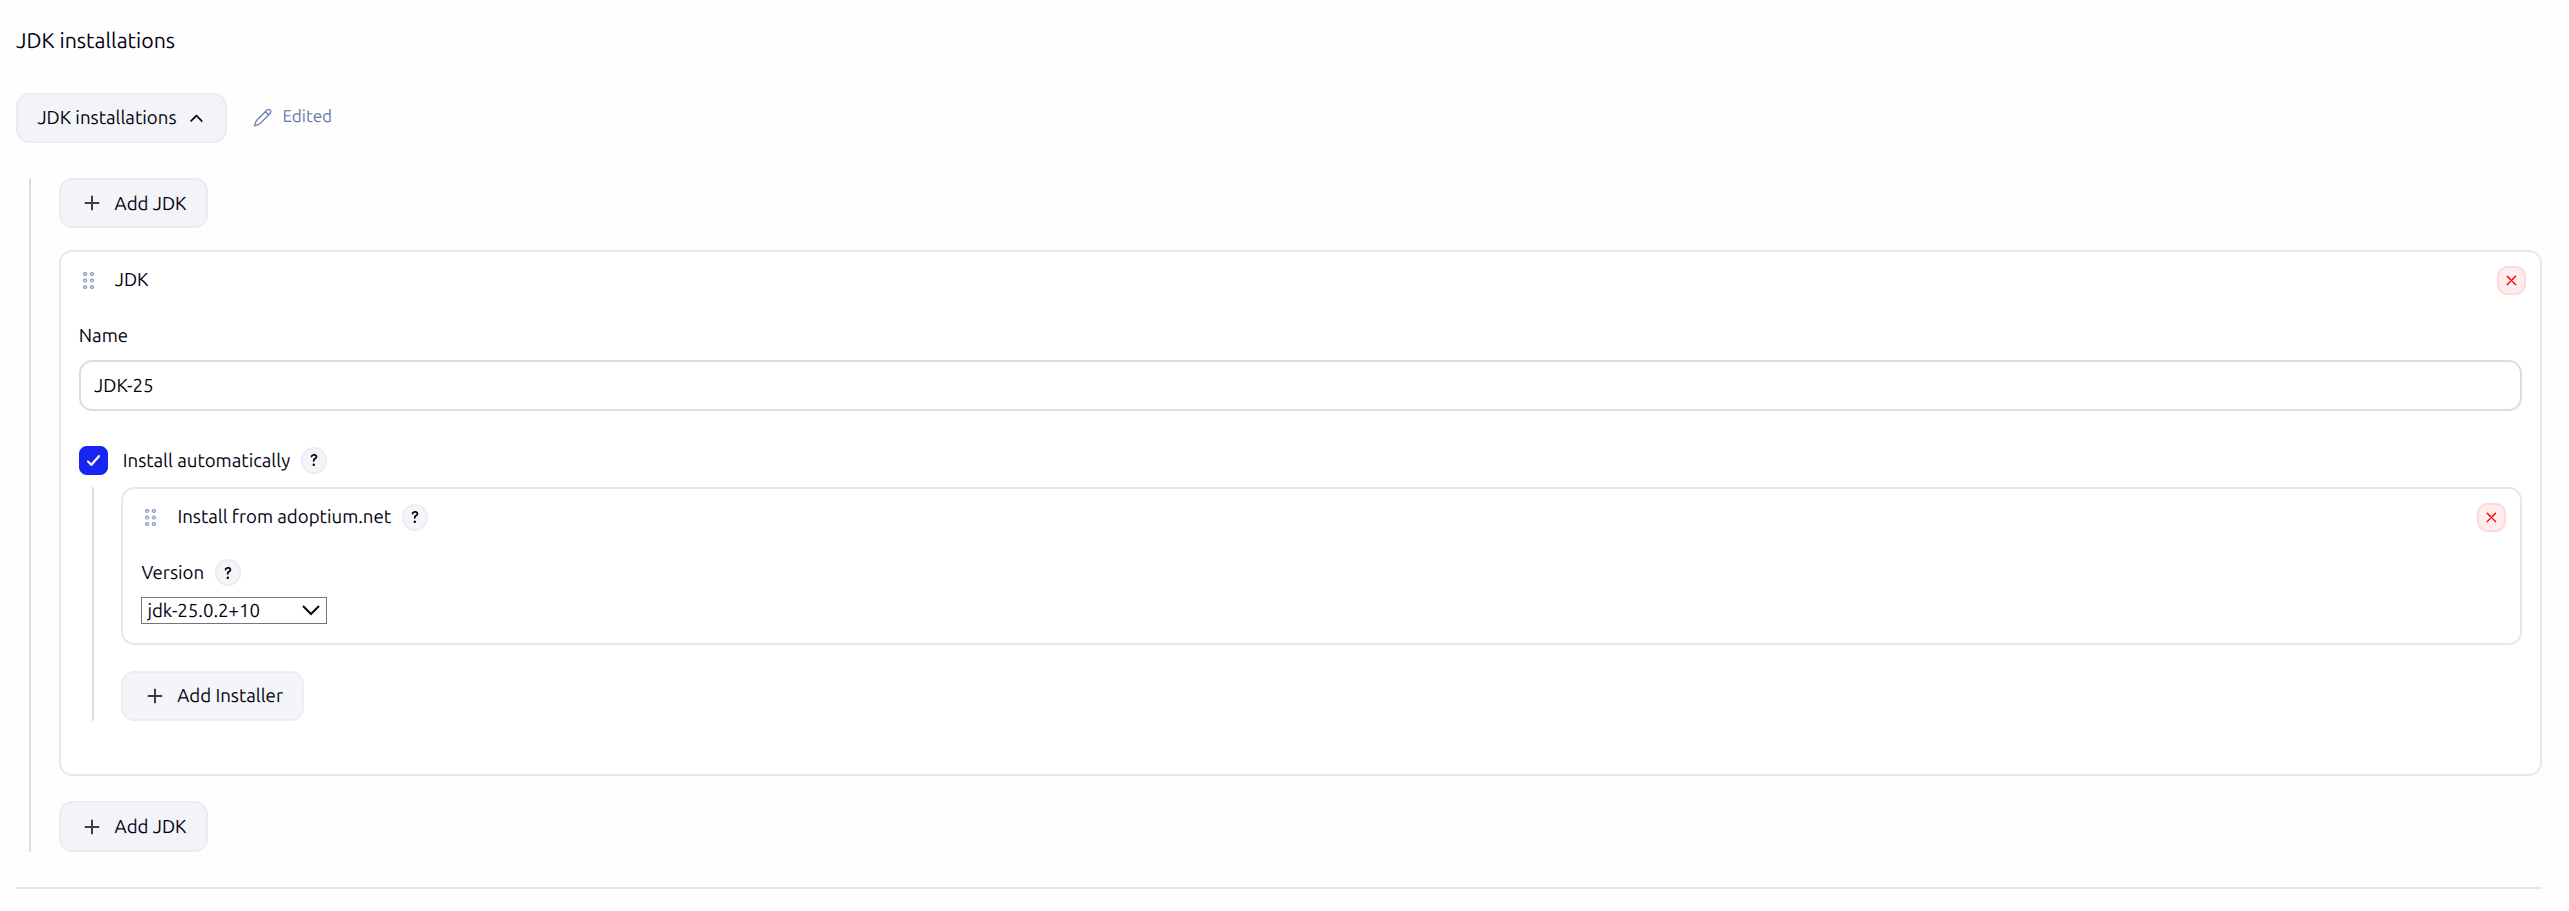
\includegraphics[width=0.9\textwidth]{img/03-jenkins-multibranch-prs.png}
    \caption{Danh sách các Pull Request được tự động phát hiện và build}
\end{figure}

\section{Chi tiết Pipeline (Jenkinsfile)}

Pipeline được viết bằng \textbf{Declarative Pipeline} trong file \texttt{Jenkinsfile} tại root của repository. Tổng cộng 298 dòng, 8 stages chính.

\subsection{Cấu hình chung}
\begin{lstlisting}[language=java, caption={Cấu hình pipeline}]
pipeline {
    agent any
    tools {
        maven 'Maven'
        jdk   'JDK-25'
    }
    options {
        timestamps()
        buildDiscarder(logRotator(numToKeepStr: '10'))
        timeout(time: 60, unit: 'MINUTES')
        disableConcurrentBuilds()
    }
    environment {
        COVERAGE_THRESHOLD = '70'
        SONAR_HOST_URL     = 'http://3.27.92.213:9000'
        MAVEN_OPTS         = '-Xmx512m -XX:MaxMetaspaceSize=256m'
    }
}
\end{lstlisting}

Các cấu hình quan trọng:
\begin{itemize}[noitemsep]
    \item \texttt{COVERAGE\_THRESHOLD = '70'}: Ngưỡng coverage tối thiểu 70\%
    \item \texttt{MAVEN\_OPTS}: Giới hạn bộ nhớ JVM để phù hợp với EC2
    \item \texttt{disableConcurrentBuilds()}: Tránh xung đột khi nhiều builds chạy cùng lúc
\end{itemize}

\subsection{Stage 1: Checkout}
\begin{lstlisting}[language=java, caption={Stage Checkout}]
stage('Checkout') {
    steps {
        checkout scm
        sh 'git fetch origin main:refs/remotes/origin/main || true'
        sh 'chmod +x ci/detect-changed-modules.sh ci/check-coverage.sh'
    }
}
\end{lstlisting}

Stage này thực hiện:
\begin{itemize}[noitemsep]
    \item Clone source code từ GitHub
    \item Fetch \texttt{origin/main} để có baseline cho việc so sánh thay đổi (fix shallow clone của Jenkins)
    \item Cấp quyền thực thi cho các CI scripts
\end{itemize}

\subsection{Stage 2: Detect Changed Modules}
\begin{lstlisting}[language=java, caption={Stage Detect Changed Modules}]
stage('Detect Changed Modules') {
    steps {
        script {
            env.CHANGED_MODULES = sh(
                script: 'ci/detect-changed-modules.sh',
                returnStdout: true
            ).trim()
        }
    }
}
\end{lstlisting}

Stage này gọi script \texttt{ci/detect-changed-modules.sh} để xác định modules nào thay đổi so với \texttt{origin/main}. Chi tiết về script được mô tả ở Mục \ref{sec:monorepo}.

\subsection{Stage 3: Gitleaks -- Secret Scan}
Quét toàn bộ source code tìm secrets/API keys bị rò rỉ. Chi tiết ở Mục \ref{sec:gitleaks}.

\subsection{Stage 4: Test (JUnit + JaCoCo)}
\begin{lstlisting}[language=java, caption={Stage Test}]
stage('Test') {
    steps {
        script {
            def modules = env.CHANGED_MODULES.split(',')
            for (module in modules) {
                sh "mvn -B -ntp -pl ${module} -am test jacoco:report -DskipITs"
            }
        }
    }
    post {
        always {
            junit allowEmptyResults: true,
                  testResults: '**/target/surefire-reports/*.xml'
            archiveArtifacts allowEmptyArchive: true,
                             artifacts: '**/target/site/jacoco/jacoco.xml'
        }
    }
}
\end{lstlisting}

Stage này:
\begin{itemize}[noitemsep]
    \item Chỉ chạy test cho \textbf{modules thay đổi} (\texttt{-pl \$\{module\}})
    \item Tự động build dependencies (\texttt{-am}: also make)
    \item Skip Integration Tests (\texttt{-DskipITs})
    \item Sinh JaCoCo coverage report (\texttt{jacoco:report})
    \item Upload test results (JUnit XML) và coverage report (JaCoCo XML) lên Jenkins
\end{itemize}

\subsection{Stage 5: Coverage Gate}
\begin{lstlisting}[language=java, caption={Stage Coverage Gate}]
stage('Coverage Gate') {
    steps {
        script {
            def modules = env.CHANGED_MODULES.split(',')
            def serviceModules = modules.findAll { it != 'common-library' }
            if (serviceModules.isEmpty()) {
                echo ">>> No service modules to check coverage"
            } else {
                for (module in serviceModules) {
                    sh "ci/check-coverage.sh ${module} ${env.COVERAGE_THRESHOLD}"
                }
            }
        }
    }
}
\end{lstlisting}

Stage này:
\begin{itemize}[noitemsep]
    \item Gọi script \texttt{ci/check-coverage.sh} để kiểm tra coverage $\geq$ 70\%
    \item \textbf{Exclude common-library}: Đây là shared library với coverage 33\% từ upstream, không phải service module
    \item Script parse JaCoCo XML report, tính LINE coverage percentage
    \item Pipeline FAIL nếu bất kỳ service module nào có coverage $<$ 70\%
\end{itemize}

\subsection{Stage 6: Build}
\begin{lstlisting}[language=java, caption={Stage Build}]
stage('Build') {
    steps {
        script {
            def modules = env.CHANGED_MODULES.split(',')
            for (module in modules) {
                sh "mvn -B -ntp -DskipTests -pl ${module} -am package"
            }
        }
    }
}
\end{lstlisting}

Build chỉ các modules thay đổi, skip tests (đã chạy ở stage 4).

\subsection{Stage 7: SonarQube Analysis}
Phân tích chất lượng code. Chi tiết ở Mục \ref{sec:sonarqube}.

\subsection{Stage 8: Snyk Dependency Scan}
Quét lỗ hổng bảo mật trong dependencies. Chi tiết ở Mục \ref{sec:snyk}.

\subsection{Post Actions}
\begin{lstlisting}[language=java, caption={Post-build actions}]
post {
    always { cleanWs() }
    success {
        echo "PIPELINE PASSED SUCCESSFULLY"
    }
    failure {
        echo "PIPELINE FAILED - Check console output"
    }
}
\end{lstlisting}

\begin{itemize}[noitemsep]
    \item \texttt{cleanWs()}: Dọn workspace sau mỗi build để tiết kiệm disk
    \item In thông báo kết quả (pass/fail) kèm branch name và build number
\end{itemize}

\section{Monorepo Path Filter}
\label{sec:monorepo}

\subsection{Vấn đề}
YAS là một monorepo chứa hơn 19 modules. Nếu mỗi lần push đều build/test \textbf{toàn bộ} modules, thời gian CI sẽ rất lâu và lãng phí tài nguyên. Cần một cơ chế chỉ build/test các modules thực sự thay đổi.

\subsection{Giải pháp: detect-changed-modules.sh}
Nhóm viết script \texttt{ci/detect-changed-modules.sh} (74 dòng) để xác định modules thay đổi so với \texttt{origin/main}.

\begin{lstlisting}[language=bash, caption={Logic chính của detect-changed-modules.sh}]
#!/usr/bin/env bash
set -euo pipefail

# Danh sach cac module cua monorepo
modules=(
  automation-ui backoffice-bff cart common-library
  customer delivery discount inventory location
  media order payment product promotion
  rating recommendation sampledata search
  storefront-bff tax webhook
)

# Lay danh sach files thay doi so voi origin/main
changed_files="$(git diff --name-only origin/main...HEAD 2>/dev/null || true)"

# Neu thay doi o root files -> build tat ca modules
if grep -Eq '^(pom\.xml|\.github/|checkstyle/|common-library/|docker/|k8s/|scripts/)' \
     <<< "${changed_files}"; then
    printf '%s\n' "${modules[@]}" | paste -sd ','
    exit 0
fi

# Map file -> module
selected_modules=()
for mod in "${modules[@]}"; do
    if grep -q "^${mod}/" <<< "${changed_files}"; then
        selected_modules+=("${mod}")
    fi
done

# Fallback: build common-library
if [[ ${#selected_modules[@]} -eq 0 ]]; then
    selected_modules=("common-library")
fi

printf '%s\n' "${selected_modules[@]}" | paste -sd ','
\end{lstlisting}

\subsection{Chiến lược phát hiện thay đổi}
\begin{table}[H]
\centering
\caption{Quy tắc phát hiện module thay đổi}
\begin{tabular}{|l|l|}
\hline
\textbf{Files thay đổi} & \textbf{Modules được build} \\
\hline
\texttt{pom.xml} (root) & Tất cả modules \\
\hline
\texttt{common-library/*} & Tất cả modules (shared dependency) \\
\hline
\texttt{media/src/*} & Chỉ \texttt{media} \\
\hline
\texttt{tax/src/*} & Chỉ \texttt{tax} \\
\hline
\texttt{ci/*}, \texttt{docs/*} & \texttt{common-library} (fallback) \\
\hline
\end{tabular}
\end{table}

\subsection{Kết quả}
\begin{itemize}[noitemsep]
    \item Thời gian build giảm đáng kể: thay vì build toàn bộ 19 modules ($\sim$30 phút), chỉ build 1--2 modules ($\sim$3--5 phút)
    \item Tiết kiệm tài nguyên AWS EC2
    \item Pipeline vẫn đảm bảo tính chính xác nhờ flag \texttt{-am} (also make dependencies)
\end{itemize}

% [Ảnh: Console output hiển thị "Modules selected for CI: media"]

\section{Unit Test và Báo cáo JaCoCo}
\label{sec:unittest}

\newcommand{\jacocofigureplaceholder}[3]{
\begin{figure}[H]
    \centering
    \IfFileExists{#1}{
        \includegraphics[width=0.92\textwidth]{#1}
    }{
        \fbox{
            \parbox[c][0.22\textheight][c]{0.86\textwidth}{
                \centering
                Ảnh JaCoCo Coverage cho module \texttt{#2}\\
                \texttt{#1}
            }
        }
    }
    \caption{#3}
\end{figure}
}

\subsection{Hướng dẫn chung chạy Unit Test}
Dự án YAS sử dụng cấu trúc monorepo Maven. Khi cần chạy test cho một service cụ thể, lệnh được thực thi từ thư mục gốc repository và truyền tên module qua tham số \texttt{-pl}. Sau khi test hoàn tất, JaCoCo sinh báo cáo tại \texttt{<module>/target/site/jacoco/index.html}.

\begin{lstlisting}[language=bash, caption={Lệnh chạy test và sinh báo cáo JaCoCo cho từng module}]
./mvnw -f pom.xml test -pl <module> -am
./mvnw -f pom.xml test jacoco:report -pl <module> -am
open <module>/target/site/jacoco/index.html
\end{lstlisting}

Quy trình trên được dùng để kiểm tra độc lập từng service trước khi đẩy Pull Request. Pipeline Jenkins cũng chạy test theo module thay đổi, upload JUnit report và xuất JaCoCo report để phục vụ bước kiểm tra coverage.

\subsection{Chi tiết Unit Test theo Service}
Tương tự format phần Unit Test của báo cáo tham khảo, mỗi service được trình bày thống nhất bằng kết quả chạy unit test và ảnh JaCoCo tương ứng. Phần này không lặp lại thông tin triển khai hoặc số liệu chi tiết vì các thông tin này đã nằm trong lịch sử Pull Request, Jenkins và JaCoCo.

\subsubsection{Module media}
\textbf{Kết quả:} Unit test chạy thành công và báo cáo JaCoCo được sinh để phục vụ kiểm tra coverage.

\jacocofigureplaceholder{img/media.png}{media}{Báo cáo JaCoCo Coverage -- module media}

\subsubsection{Module product}
\textbf{Kết quả:} Unit test chạy thành công và báo cáo JaCoCo được sinh để phục vụ kiểm tra coverage.

\jacocofigureplaceholder{img/product.png}{product}{Báo cáo JaCoCo Coverage -- module product}

\subsubsection{Module order}
\textbf{Kết quả:} Unit test chạy thành công và báo cáo JaCoCo được sinh để phục vụ kiểm tra coverage.

\jacocofigureplaceholder{img/order.png}{order}{Báo cáo JaCoCo Coverage -- module order}

\subsubsection{Module inventory}
\textbf{Kết quả:} Unit test chạy thành công và báo cáo JaCoCo được sinh để phục vụ kiểm tra coverage.

\jacocofigureplaceholder{img/inventory.png}{inventory}{Báo cáo JaCoCo Coverage -- module inventory}

\subsubsection{Module payment}
\textbf{Kết quả:} Unit test chạy thành công và báo cáo JaCoCo được sinh để phục vụ kiểm tra coverage.

\jacocofigureplaceholder{img/payment.png}{payment}{Báo cáo JaCoCo Coverage -- module payment}

\subsubsection{Module payment-paypal}
\textbf{Kết quả:} Unit test chạy thành công và báo cáo JaCoCo được sinh để phục vụ kiểm tra coverage.

\jacocofigureplaceholder{img/payment-paypal.png}{payment-paypal}{Báo cáo JaCoCo Coverage -- module payment-paypal}

\subsubsection{Module promotion}
\textbf{Kết quả:} Unit test chạy thành công và báo cáo JaCoCo được sinh để phục vụ kiểm tra coverage.

\jacocofigureplaceholder{img/promotion.png}{promotion}{Báo cáo JaCoCo Coverage -- module promotion}

\subsubsection{Module rating}
\textbf{Kết quả:} Unit test chạy thành công và báo cáo JaCoCo được sinh để phục vụ kiểm tra coverage.

\jacocofigureplaceholder{img/rating.png}{rating}{Báo cáo JaCoCo Coverage -- module rating}

\subsubsection{Module delivery}
\textbf{Kết quả:} Unit test chạy thành công và báo cáo JaCoCo được sinh để phục vụ kiểm tra coverage.

\jacocofigureplaceholder{img/delivery.png}{delivery}{Báo cáo JaCoCo Coverage -- module delivery}

\subsubsection{Module recommendation}
\textbf{Kết quả:} Unit test chạy thành công và báo cáo JaCoCo được sinh để phục vụ kiểm tra coverage.

\jacocofigureplaceholder{img/recommendation.png}{recommendation}{Báo cáo JaCoCo Coverage -- module recommendation}

\subsubsection{Module customer}
\textbf{Kết quả:} Unit test chạy thành công và báo cáo JaCoCo được sinh để phục vụ kiểm tra coverage.

\jacocofigureplaceholder{img/customer.png}{customer}{Báo cáo JaCoCo Coverage -- module customer}

\subsubsection{Module location}
\textbf{Kết quả:} Unit test chạy thành công và báo cáo JaCoCo được sinh để phục vụ kiểm tra coverage.

\jacocofigureplaceholder{img/location.png}{location}{Báo cáo JaCoCo Coverage -- module location}

\subsubsection{Module cart}
\textbf{Kết quả:} Unit test chạy thành công và báo cáo JaCoCo được sinh để phục vụ kiểm tra coverage.

\jacocofigureplaceholder{img/cart.png}{cart}{Báo cáo JaCoCo Coverage -- module cart}

\subsubsection{Module tax}
\textbf{Kết quả:} Unit test chạy thành công và báo cáo JaCoCo được sinh để phục vụ kiểm tra coverage.

\jacocofigureplaceholder{img/tax.png}{tax}{Báo cáo JaCoCo Coverage -- module tax}

\subsubsection{Module webhook}
\textbf{Kết quả:} Unit test chạy thành công và báo cáo JaCoCo được sinh để phục vụ kiểm tra coverage.

\jacocofigureplaceholder{img/webhook.png}{webhook}{Báo cáo JaCoCo Coverage -- module webhook}

\subsection{Coverage Gate trong Jenkins}
Coverage Gate được đặt tại pipeline để bảo đảm mỗi PR không chỉ chạy pass unit test mà còn tạo được báo cáo độ phủ. Script \texttt{ci/check-coverage.sh} đọc chỉ số LINE coverage từ file \texttt{jacoco.xml} của module và so sánh với ngưỡng cấu hình.

\begin{lstlisting}[language=bash, caption={check-coverage.sh -- kiểm tra ngưỡng coverage}]
module="$1"
minimum="$2"
report_path="${module}/target/site/jacoco/jacoco.xml"

line_counter="$(grep '<counter type="LINE"' "${report_path}" | tail -1)"
covered="$(echo "${line_counter}" | sed 's/.*covered="\([0-9]*\)".*/\1/')"
missed="$(echo "${line_counter}" | sed 's/.*missed="\([0-9]*\)".*/\1/')"

total=$((covered + missed))
coverage_percent="$(awk -v c="${covered}" -v t="${total}" \
    'BEGIN { printf "%.2f", (c / t) * 100 }')"

awk -v actual="${coverage_percent}" -v threshold="${minimum}" \
    'BEGIN { exit !(actual + 0 >= threshold + 0) }'
\end{lstlisting}

\begin{itemize}[noitemsep]
    \item \textbf{Ngưỡng kiểm tra}: cấu hình qua biến \texttt{COVERAGE\_THRESHOLD}.
    \item \textbf{Mức đọc dữ liệu}: dùng counter \texttt{LINE} cấp report-level trong \texttt{jacoco.xml}.
    \item \textbf{Tích hợp Jenkins}: nếu coverage thấp hơn ngưỡng, stage Coverage Gate trả lỗi và pipeline thất bại.
    \item \textbf{Minh chứng}: console log Jenkins hiển thị module được kiểm tra, phần trăm coverage thực tế và kết quả pass/fail.
\end{itemize}

\begin{figure}[H]
    \centering
    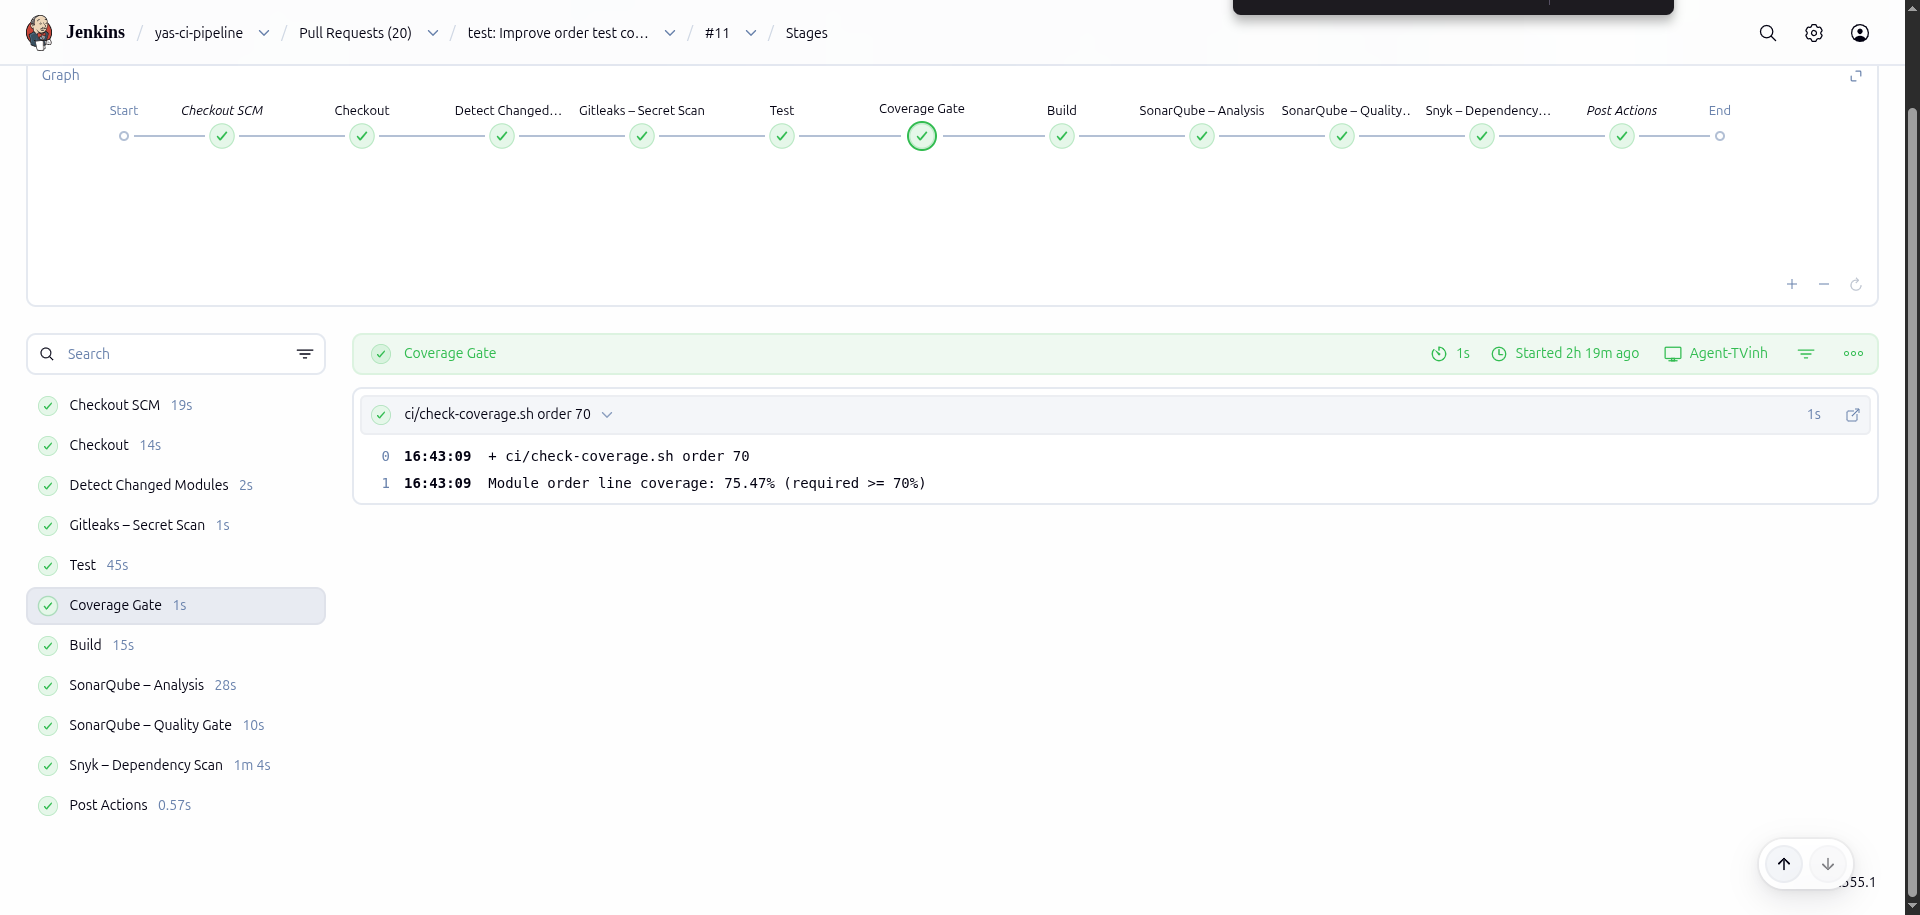
\includegraphics[width=0.92\textwidth]{img/10-jenkins-console-coverage-gate.png}
    \caption{Console output Jenkins khi kiểm tra ngưỡng Coverage Gate}
\end{figure}

\section{Gitleaks -- Secret Scanning}
\label{sec:gitleaks}

\subsection{Vấn đề}
Repository YAS chứa nhiều file cấu hình Kubernetes và Docker từ upstream, trong đó có các chuỗi base64-encoded trông giống API keys hoặc secrets. Cần phân biệt giữa \textbf{secrets thật sự mới} (do nhóm vô tình commit) và \textbf{false positives} từ upstream.

\subsection{Công cụ: Gitleaks v8.18.4}
Gitleaks là công cụ mã nguồn mở chuyên quét secrets trong source code. Nhóm sử dụng phiên bản 8.18.4 với chế độ \texttt{--no-git} (quét file trực tiếp, không cần git history).

\subsection{Cấu hình}

\subsubsection{gitleaks.toml}
File cấu hình chính, extend từ bộ rules mặc định và thêm allowlist cho các đường dẫn an toàn:

\begin{lstlisting}[language=bash, caption={gitleaks.toml}]
[extend]
useDefault = true

[allowlist]
paths = [
    '''k8s/.*''',
    '''docker/.*''',
    '''automation-ui/.*''',
    '''.github/.*''',
    '''scripts/.*''',
    '''.*\.md$''',
    '''.*\.json$''',
    '''gitleaks-baseline\.json''',
    '''gitleaks-report\.json'''
]
\end{lstlisting}

\subsubsection{.gitleaksignore}
File chứa danh sách 13 fingerprints cụ thể của các secrets từ upstream cần bỏ qua:

\begin{lstlisting}[caption={.gitleaksignore (trích)}]
# Upstream K8s secrets
6abd7e0e...  # k8s/base secrets
a7f12cb3...  # docker compose credentials
# ... (13 entries)
\end{lstlisting}

\subsubsection{gitleaks-baseline.json}
Baseline trống (\texttt{[]}), đảm bảo chỉ phát hiện secrets \textbf{mới} so với baseline.

\subsection{Luồng quét trong Pipeline}
\begin{enumerate}[noitemsep]
    \item Tải Gitleaks binary (cache nếu đã có)
    \item Kiểm tra baseline file tồn tại
    \item Chạy quét với \texttt{--no-git --config=gitleaks.toml --baseline-path=gitleaks-baseline.json}
    \item Nếu phát hiện secret mới → \textbf{Pipeline FAIL} (\texttt{--exit-code=1})
    \item Nếu không phát hiện → In ``Gitleaks scan PASSED''
\end{enumerate}

\subsection{Kết quả}
\begin{itemize}[noitemsep]
    \item Tất cả các build đều pass Gitleaks scan
    \item 13 false positives từ upstream đã được xử lý qua \texttt{.gitleaksignore}
    \item Console output: \texttt{>>> Gitleaks scan PASSED - no new secrets found}
\end{itemize}

\begin{figure}[H]
    \centering
    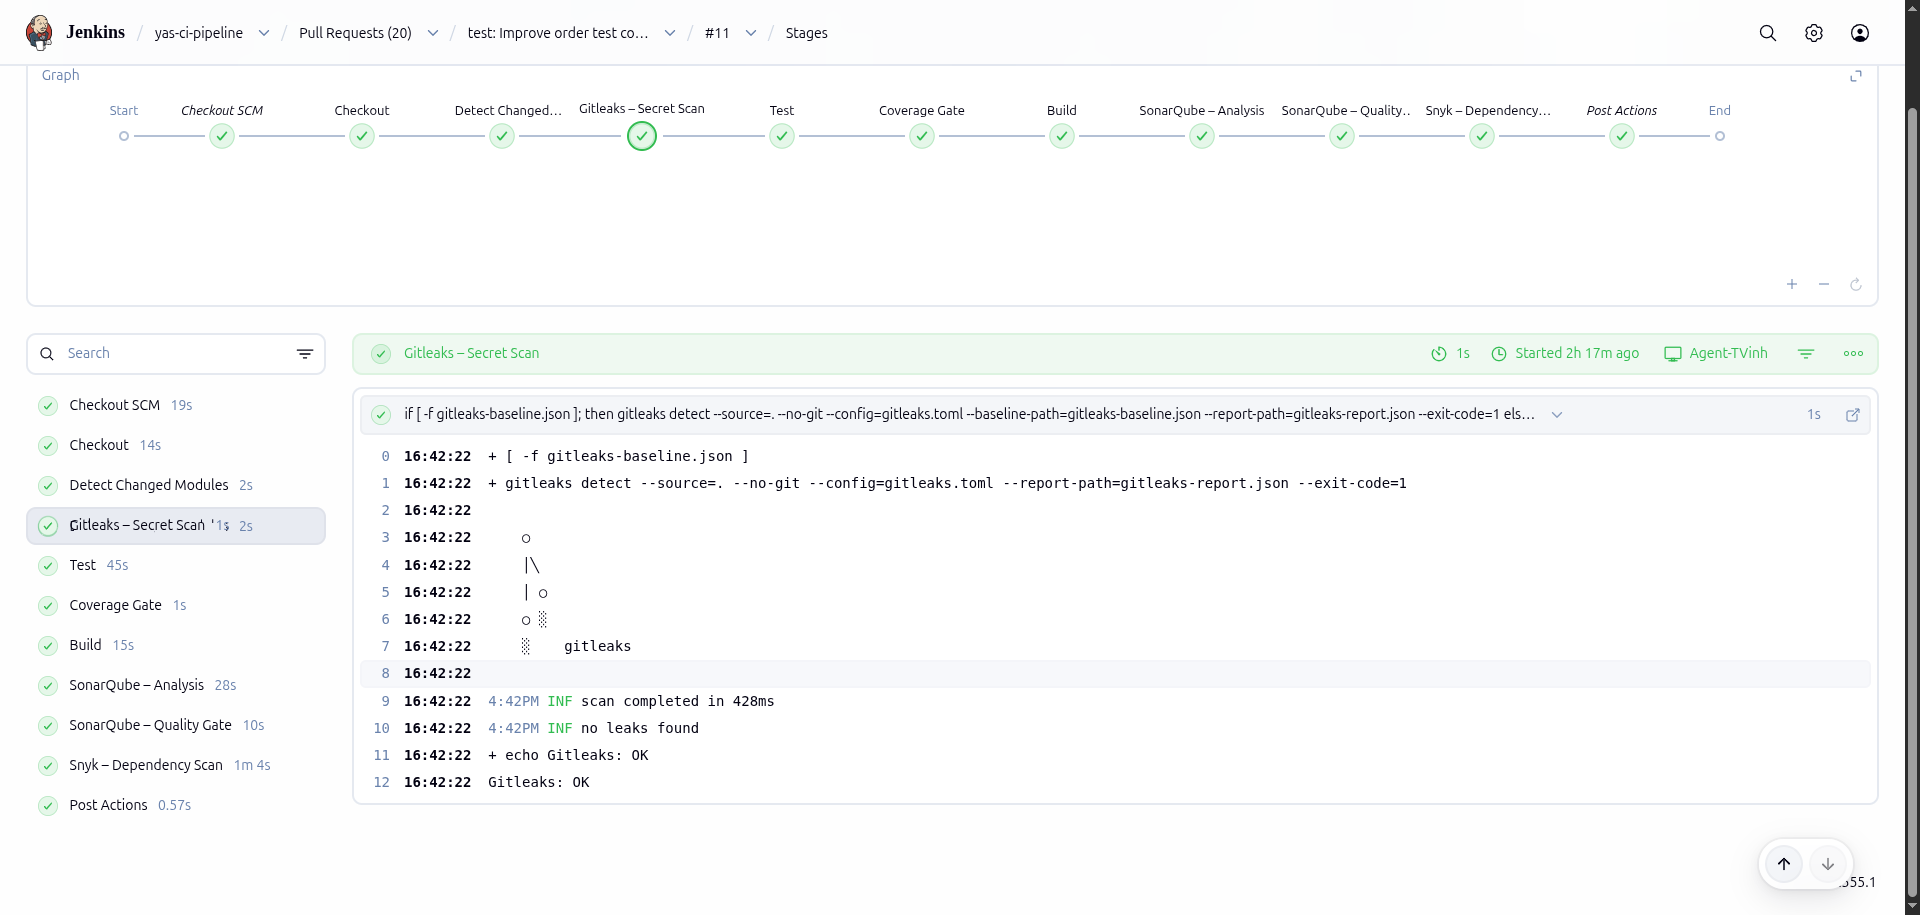
\includegraphics[width=0.9\textwidth]{img/08-jenkins-console-gitleaks-pass.png}
    \caption{Console output hiển thị Gitleaks quét thành công (không phát hiện rò rỉ secret)}
\end{figure}

\section{SonarQube -- Code Quality Analysis}
\label{sec:sonarqube}

\subsection{Giới thiệu}
SonarQube là nền tảng phân tích chất lượng code, phát hiện bugs, code smells, security vulnerabilities và đo lường coverage.

Nhóm sử dụng SonarQube \textbf{self-hosted} trên cùng AWS EC2 instance với Jenkins, truy cập tại \texttt{http://3.27.92.213:9000}.

\subsection{Cấu hình Server}
\begin{itemize}[noitemsep]
    \item \textbf{SonarQube URL}: \texttt{http://3.27.92.213:9000}
    \item \textbf{Authentication}: Token-based, lưu trong Jenkins Credentials (\texttt{sonarqube-token})
    \item \textbf{Project Key}: \texttt{nashtech-garage\_yas-yas-parent} (auto-detected từ pom.xml)
\end{itemize}

% [Ảnh: Screenshot cấu hình Jenkins System - SonarQube servers]
% [Ảnh: Screenshot cấu hình Webhook trên SonarQube]
% [Ảnh: SonarQube Dashboard - Overview]

\subsection{Tích hợp trong Pipeline}
\begin{lstlisting}[language=java, caption={SonarQube Analysis \& Quality Gate}]
stage('SonarQube - Analysis') {
    steps {
        withSonarQubeEnv('sonar-server') {
            withCredentials([string(credentialsId: 'sonarqube-token', variable: 'SONAR_TOKEN')]) {
                sh "mvn sonar:sonar -pl ${plArg} -am -Dsonar.host.url=..."
            }
        }
    }
}
stage('SonarQube - Quality Gate') {
    steps {
        withSonarQubeEnv('sonar-server') {
            timeout(time: 15, unit: 'MINUTES') {
                waitForQualityGate abortPipeline: false
            }
        }
    }
}
\end{lstlisting}

\subsection{Thiết kế và Quality Gate}
\begin{itemize}[noitemsep]
    \item Chỉ phân tích \textbf{service modules} thay đổi (exclude common-library)
    \item Sử dụng \texttt{withSonarQubeEnv} để Jenkins tự động nhận biết cấu hình server.
    \item Stage \textbf{Quality Gate} sử dụng lệnh \texttt{waitForQualityGate} để treo Pipeline cho đến khi SonarQube phân tích xong và gửi webhook kết quả về lại Jenkins.
\end{itemize}

\subsection{Kết quả}
\begin{itemize}[noitemsep]
    \item Console: \texttt{[INFO] ANALYSIS SUCCESSFUL}
    \item SonarQube task URL được in ra để truy cập dashboard
    \item Dashboard hiển thị: bugs, vulnerabilities, code smells, coverage percentage, duplications
\end{itemize}

% [Ảnh: SonarQube Dashboard - Project overview (bugs, coverage, smells)]
% [Ảnh: Console output "[INFO] ANALYSIS SUCCESSFUL"]

\section{Snyk -- Dependency Vulnerability Scan}
\label{sec:snyk}

\subsection{Giới thiệu}
Snyk là công cụ quét lỗ hổng bảo mật trong dependencies (thư viện phụ thuộc). Nhóm tích hợp Snyk CLI vào pipeline để tự động phát hiện các thư viện có CVE (Common Vulnerabilities and Exposures).

\subsection{Cấu hình}
\begin{itemize}[noitemsep]
    \item \textbf{Snyk CLI}: Cài đặt trên Jenkins server
    \item \textbf{Authentication}: Token-based, lưu trong Jenkins Credentials (\texttt{snyk-token})
    \item \textbf{Severity threshold}: \texttt{high} --- chỉ báo cáo lỗ hổng mức high trở lên
\end{itemize}

\subsection{Tích hợp trong Pipeline}
Stage Snyk thực hiện 2 bước cho mỗi service module:

\subsubsection{Snyk Test}
Quét dependencies và báo cáo lỗ hổng:
\begin{lstlisting}[language=bash, caption={Snyk Test command}]
snyk test \
  --file=${module}/pom.xml \
  --severity-threshold=high \
  --all-sub-projects
\end{lstlisting}

\subsubsection{Snyk Monitor}
Đẩy snapshot dependencies lên Snyk dashboard để theo dõi liên tục:
\begin{lstlisting}[language=bash, caption={Snyk Monitor command}]
snyk monitor \
  --file=${module}/pom.xml \
  --project-name=yas-${module}
\end{lstlisting}

\subsection{Xử lý lỗi}
Pipeline được thiết kế với cơ chế \textbf{retry} và \textbf{graceful degradation}:
\begin{enumerate}[noitemsep]
    \item Chạy \texttt{snyk test} lần 1
    \item Nếu fail → retry với \texttt{--max-depth=3} (giảm độ sâu dependency tree)
    \item Nếu vẫn fail → ghi warning, pipeline \textbf{tiếp tục} (không block)
\end{enumerate}

\subsection{Khắc phục lỗi phân giải Dependency (SNYK-CLI-0000)}
Trong quá trình triển khai, nhóm từng gặp lỗi Snyk crash với mã \texttt{exit code: -13} (SNYK-CLI-0000) khi chạy trên môi trường Jenkins. 

\textbf{Nguyên nhân}: Snyk nội bộ sử dụng \texttt{mvn dependency:tree} để phân tích. Với kiến trúc Monorepo, việc quét một module con (ví dụ \texttt{order}) bằng cờ \texttt{-f order/pom.xml} sẽ khiến Maven không tìm thấy file POM cha (\texttt{yas} parent) để nội suy biến \texttt{\$\{revision\}}, dẫn đến việc tiến trình cấp dưới của Snyk bị lỗi và trả về mã -13.

\textbf{Cách giải quyết}: Nhóm đã cấu hình lại Pipeline để chạy lệnh \texttt{mvn dependency:tree -pl \$\{module\} -am} trước bước chạy Snyk. Lệnh này giúp Maven tải và cache sẵn toàn bộ dependency tree của module và POM cha vào local repository. Nhờ vậy, bước quét Snyk sau đó diễn ra hoàn toàn trơn tru và không còn lỗi.

% [Ảnh: Console output Snyk scanning]
% [Ảnh: Giao diện Snyk Web Dashboard]

\section{Kết quả thực thi Pipeline}

\subsection{Danh sách Pull Requests}
\begin{table}[H]
\centering
\caption{Danh sách Pull Requests trên GitHub}
\begin{tabular}{|c|l|l|l|}
\hline
\textbf{PR} & \textbf{Title} & \textbf{Branch} & \textbf{Trạng thái} \\
\hline
\#5 & ci: setup Jenkins pipeline & ci/setup-jenkins-pipeline & Merged \\
\hline
\#6 & test(tax): add coverage & tri/tax-tests & Open (CI pass) \\
\hline
\#7 & test(media): add coverage & feature/media-tests & Open (CI pass) \\
\hline
\#8 & fix(ci): coverage gate bug & ci/setup-jenkins-pipeline & Open \\
\hline
\end{tabular}
\end{table}

% [Ảnh: GitHub Pull Requests list]

\subsection{Kết quả Pipeline cho PR \#7 (media)}
\begin{table}[H]
\centering
\caption{Kết quả pipeline PR \#7 - Module media}
\begin{tabular}{|l|l|l|}
\hline
\textbf{Stage} & \textbf{Kết quả} & \textbf{Thời gian} \\
\hline
Checkout SCM & \textcolor{green}{PASS} & 7s \\
\hline
Tool Install & \textcolor{green}{PASS} & 0.22s \\
\hline
Checkout & \textcolor{green}{PASS} & 4s \\
\hline
Detect Changed Modules & \textcolor{green}{PASS} & 0.74s \\
\hline
Gitleaks -- Secret Scan & \textcolor{green}{PASS} & 2s \\
\hline
Test & \textcolor{green}{PASS} (36 tests, 0 failures) & 74s \\
\hline
Coverage Gate & \textcolor{green}{PASS} & --- \\
\hline
Build & \textcolor{green}{PASS} & 82ms \\
\hline
SonarQube -- Analysis & \textcolor{green}{PASS} & 10min \\
\hline
Snyk -- Dependency Scan & Warning (exit -13) & 45s \\
\hline
\end{tabular}
\end{table}

% [Ảnh: Jenkins Pipeline Stage View - PR #7 (tất cả stages xanh)]
% [Ảnh: Console output PR #7 - "Tests run: 36, Failures: 0"]

\subsection{Kết quả Pipeline cho PR \#6 (tax)}
\begin{table}[H]
\centering
\caption{Kết quả pipeline PR \#6 - Module tax}
\begin{tabular}{|l|l|l|}
\hline
\textbf{Stage} & \textbf{Kết quả} & \textbf{Thời gian} \\
\hline
Checkout SCM & \textcolor{green}{PASS} & --- \\
\hline
Detect Changed Modules & \textcolor{green}{PASS} & --- \\
\hline
Gitleaks -- Secret Scan & \textcolor{green}{PASS} & --- \\
\hline
Test & \textcolor{green}{PASS} (47 tests, 0 failures) & --- \\
\hline
Coverage Gate & \textcolor{green}{PASS} & --- \\
\hline
Build & \textcolor{green}{PASS} & --- \\
\hline
SonarQube -- Analysis & \textcolor{green}{PASS} & --- \\
\hline
Snyk -- Dependency Scan & Warning (exit -13) & --- \\
\hline
\end{tabular}
\end{table}

% [Ảnh: Jenkins Pipeline Stage View - PR #6]
% [Ảnh: Console output PR #6 - "Tests run: 47, Failures: 0"]

\subsection{Minh chứng Branch Protection hoạt động}
Trên mỗi Pull Request, GitHub hiển thị:
\begin{enumerate}[noitemsep]
    \item \textbf{Review required}: ``At least 2 approving reviews are required''
    \item \textbf{Status checks}: CI pipeline phải pass trước khi merge
    \item \textbf{Merge blocked}: Nút ``Merge'' bị disabled khi chưa đủ conditions
\end{enumerate}

% [Ảnh: GitHub PR hiển thị "Review required" + "Checks passed"]
% [Ảnh: GitHub PR hiển thị "Merging is blocked" khi chưa đủ approvals]

\section{Phân công công việc}

\subsection{Thành viên nhóm}
\begin{table}[H]
\centering
\caption{Thông tin thành viên nhóm}
\begin{tabular}{|l|l|l|}
\hline
\textbf{Họ tên} & \textbf{MSSV} & \textbf{Vai trò} \\
\hline
Nguyễn Lê Thế Vinh & [MSSV1] & Leader \\
\hline
Phạm Quang Vinh & [MSSV2] & Infra \& Security \\
\hline
Lê Xuân Trí & [MSSV3] & Testing \\
\hline
\end{tabular}
\end{table}

\subsection{Chi tiết phân công}

\subsubsection{Nguyễn Lê Thế Vinh (Leader)}
\begin{itemize}[noitemsep]
    \item Fork repository, thêm collaborators
    \item Viết \texttt{Jenkinsfile} (8 stages, 298 dòng)
    \item Viết \texttt{ci/detect-changed-modules.sh} (monorepo path filter)
    \item Viết \texttt{ci/check-coverage.sh} (coverage gate $\geq$ 70\%)
    \item Cấu hình \texttt{gitleaks.toml}, \texttt{.gitleaksignore}, \texttt{gitleaks-baseline.json}
    \item Cấu hình GitHub Rulesets (branch protection)
    \item Debug và fix awk parsing bug trong coverage gate
    \item Viết báo cáo
    \item Review và approve PRs
\end{itemize}

\subsubsection{Phạm Quang Vinh (Infra \& Security)}
\begin{itemize}[noitemsep]
    \item Setup AWS EC2 instance
    \item Cài đặt và cấu hình Jenkins server
    \item Cài đặt và cấu hình SonarQube server
    \item Cài đặt Snyk CLI trên Jenkins server
    \item Cấu hình Jenkins Credentials (SonarQube token, Snyk token)
    \item Cấu hình Jenkins Global Tools (JDK-25, Maven)
    \item Tạo Multibranch Pipeline job
    \item Cấu hình Webhook GitHub → Jenkins
    \item Review và approve PRs
\end{itemize}

\subsubsection{Lê Xuân Trí (Testing)}
\begin{itemize}[noitemsep]
    \item Viết unit tests cho module \textbf{media} (PR \#7)
    \begin{itemize}
        \item MediaServiceUnitTest
        \item FileSystemRepositoryTest
    \end{itemize}
    \item Viết unit tests cho module \textbf{tax} (PR \#6)
    \begin{itemize}
        \item TaxRateServiceTest
        \item TaxClassServiceTest
        \item TaxRateControllerTest
    \end{itemize}
    \item Đảm bảo coverage $\geq$ 70\% cho từng module
    \item Tạo Pull Requests theo quy trình
    \item Review và approve PRs
\end{itemize}

\subsection{Tổng kết đóng góp}
\begin{table}[H]
\centering
\caption{Tổng kết đóng góp theo thành viên}
\begin{tabular}{|l|c|c|c|}
\hline
\textbf{Hạng mục} & \textbf{Vinh.NL} & \textbf{Vinh.PQ} & \textbf{Trí} \\
\hline
Pipeline (Jenkinsfile) & $\checkmark$ & & \\
\hline
CI Scripts & $\checkmark$ & & \\
\hline
Security Config & $\checkmark$ & $\checkmark$ & \\
\hline
Infrastructure & & $\checkmark$ & \\
\hline
Jenkins Setup & & $\checkmark$ & \\
\hline
SonarQube Setup & & $\checkmark$ & \\
\hline
Unit Tests -- media & & & $\checkmark$ \\
\hline
Unit Tests -- tax & & & $\checkmark$ \\
\hline
Branch Protection & $\checkmark$ & & \\
\hline
Code Review & $\checkmark$ & $\checkmark$ & $\checkmark$ \\
\hline
Báo cáo & $\checkmark$ & & \\
\hline
\end{tabular}
\end{table}

\section{Kết luận}

\subsection{Tổng kết}
Nhóm đã hoàn thành việc xây dựng hệ thống CI cho dự án YAS (Yet Another Shop) với đầy đủ các yêu cầu:

\begin{table}[H]
\centering
\caption{Checklist yêu cầu đồ án}
\begin{tabular}{|c|l|c|}
\hline
\textbf{STT} & \textbf{Yêu cầu} & \textbf{Trạng thái} \\
\hline
1 & Sử dụng Jenkins & $\checkmark$ \\
\hline
2 & Fork repo YAS & $\checkmark$ \\
\hline
3 & Branch protection (2 approvals + CI pass) & $\checkmark$ \\
\hline
4 & Jenkins quét từng branch & $\checkmark$ \\
\hline
5 & Pipeline $\geq$ 2 phases (test + build) + coverage & $\checkmark$ \\
\hline
6 & Monorepo path filter & $\checkmark$ \\
\hline
7a & Thêm unit test cho $\geq$ 2 services & $\checkmark$ \\
\hline
7b & Coverage gate $\geq$ 70\% & $\checkmark$ \\
\hline
7c & Security scanning (Gitleaks + SonarQube + Snyk) & $\checkmark$ \\
\hline
\end{tabular}
\end{table}

\subsection{Điểm nổi bật}
\begin{enumerate}[noitemsep]
    \item \textbf{Pipeline 8 stages}: Thiết kế pipeline đầy đủ từ checkout đến security scanning, mỗi stage có mục đích rõ ràng
    \item \textbf{Monorepo-aware}: Path filter thông minh giúp giảm thời gian build từ $\sim$30 phút xuống $\sim$5 phút
    \item \textbf{Coverage Gate thực sự enforce}: Parse JaCoCo XML report và so sánh với ngưỡng 70\%, pipeline FAIL nếu không đạt
    \item \textbf{Gitleaks với baseline}: Xử lý 13 false positives từ upstream bằng \texttt{.gitleaksignore} và baseline, chỉ phát hiện secrets mới
    \item \textbf{Retry mechanism cho Snyk}: Tự động retry với \texttt{--max-depth=3} nếu lần quét đầu fail
    \item \textbf{Graceful degradation}: Pipeline không bị block bởi các lỗi infrastructure (Snyk OOM, shallow clone), nhưng vẫn báo warning
\end{enumerate}

\subsection{Khó khăn gặp phải}
\begin{enumerate}[noitemsep]
    \item \textbf{Shallow clone}: Jenkins Multibranch Pipeline mặc định dùng shallow clone, khiến \texttt{git diff} không hoạt động. Fix bằng \texttt{git fetch origin main}.
    \item \textbf{Upstream secrets}: Repository gốc chứa nhiều K8s secrets dạng base64, gây false positives cho Gitleaks. Fix bằng \texttt{.gitleaksignore} + \texttt{gitleaks.toml} allowlist.
    \item \textbf{Awk parsing bug}: Script coverage gate ban đầu dùng awk nhưng logic so sánh field không đúng, dẫn đến coverage gate luôn skip. Fix bằng \texttt{grep + sed}.
    \item \textbf{Snyk OOM}: EC2 instance thiếu RAM khiến Snyk CLI bị kill (exit -13). Workaround bằng retry + graceful degradation.
    \item \textbf{Jenkins branch status pending}: Multibranch Pipeline disable branch builds khi branch đã có PR, khiến status ``branch'' kẹt pending trên GitHub. Đây là known behavior, không ảnh hưởng merge.
\end{enumerate}

\subsection{Hướng phát triển}
\begin{itemize}[noitemsep]
    \item Thêm \textbf{CD (Continuous Deployment)}: Tự động deploy lên staging/production
    \item Tăng coverage cho \textbf{tất cả service modules}, không chỉ media và tax
    \item Fix Snyk OOM bằng cách nâng cấp EC2 instance
    \item Thêm \textbf{DAST} (Dynamic Application Security Testing) cho các API endpoints
    \item Tích hợp \textbf{Slack/Discord notification} khi pipeline fail
\end{itemize}


% References
\cleardoublepage
\phantomsection
\addcontentsline{toc}{section}{Tài liệu tham khảo}

\begin{thebibliography}{9}

\bibitem{yas}
NashTech Garage, ``YAS: Yet Another Shop,''
\url{https://github.com/nashtech-garage/yas}

\bibitem{jenkins}
Jenkins, ``Jenkins User Documentation,''
\url{https://www.jenkins.io/doc/}

\bibitem{gitleaks}
Gitleaks, ``Gitleaks - Protect and discover secrets,''
\url{https://github.com/gitleaks/gitleaks}

\bibitem{sonarqube}
SonarSource, ``SonarQube Documentation,''
\url{https://docs.sonarqube.org/latest/}

\bibitem{snyk}
Snyk, ``Snyk CLI Documentation,''
\url{https://docs.snyk.io/snyk-cli}

\bibitem{jacoco}
EclEmma, ``JaCoCo Java Code Coverage Library,''
\url{https://www.jacoco.org/jacoco/}

\bibitem{multibranch}
Jenkins, ``Pipeline Multibranch,''
\url{https://www.jenkins.io/doc/book/pipeline/multibranch/}

\end{thebibliography}

\end{document}